\documentclass[a4paper,11pt]{article}
% ---- graphiques
\usepackage[pdftex]{graphicx}
\usepackage{wrapfig}
\usepackage{color}
%\usepackage{hyperref}

% for latex2html
\usepackage{html}

% for accents
\usepackage[latin1]{inputenc}
\usepackage[T1]{fontenc}

\usepackage{algorithm}
\usepackage{algorithmic}

\definecolor{darkgreen}{rgb}{0,0.4,0}
\definecolor{darkblue}{rgb}{0,0,0.4}
\definecolor{darkgray}{rgb}{0.2,0.2,0.2}

% ---- inclusion de codes
\usepackage{listings}
\lstset{showstringspaces=false,tabsize=4,basicstyle=\scriptsize\sffamily,breaklines=true,breakatwhitespace=true,framexleftmargin=5mm, frame=shadowbox, framesep=1pt,rulesepcolor=\color{darkgray},rulesep=.5pt,keywordstyle=\bf\color{blue},commentstyle=\color{magenta},stringstyle=\color{red},numbers=left,numberstyle=\tiny,numbersep=5pt,columns=flexible}

\lstdefinestyle{bash}{language=bash}
\lstdefinestyle{Perl}{language=Perl}
\lstdefinestyle{C++}{language=C++,emph={__global__,__shared__,__syncthreads,blockIdx,threadIdx,float3,float4},emphstyle=\bf\color{darkgreen}}
\lstdefinestyle{DTD}{language=XML}
\lstdefinestyle{XML}{language=XML,usekeywordsintag=false,markfirstintag=true}
%begin{latexonly}
\newcommand{\includecode}[2]{
\lstinputlisting[style=#1]{#2}
}
%end{latexonly}
\begin{htmlonly}
\newcommand{\includecode}[2]{  \htmladdnormallink{#2}{../../#2} }
\end{htmlonly}

%\lstnewenvironment{code}{}{}
\lstnewenvironment{code_bash}{\lstset{style=bash}}{}
\lstnewenvironment{code_perl}{\lstset{style=Perl}}{}
\lstnewenvironment{code_cpp}{\lstset{style=C++}}{}
\lstnewenvironment{code_dtd}{\lstset{style=DTD}}{}
\lstnewenvironment{code_xml}{\lstset{style=XML}}{}

\newcommand{\textcode}[1]{{\sf #1}}



%
\newcommand{\sofa}{SOFA}
\newcommand{\todo}[1]{}
\newcommand{\eg}{\textit{e.g.} }

\renewcommand{\vec}[1]{\ensuremath{\mathbf{#1 }}} % vector
\newcommand{\Vx}{\vec{x} } % position vector
\newcommand{\Vv}{\vec{v} } % velocity vector
\newcommand{\Va}{\vec{a} } % acceleration vector
\newcommand{\Vf}{\vec{f}} % force
\newcommand{\Vdv}{\vec{\delta\Vv}} % change of velocity vector (unknown in implicit CG, and used in constraint solver
\renewcommand{\P}{\mat{P} } % projection to a constrained space.

\newcommand{\JNL}{\mathbf{\mathcal{J}} }     % mapping des positions
\newcommand{\J}{\mat J }                 % mapping lineaire
\newcommand{\M}{\mat M }             % matrice de masse
\newcommand{\K}{\mat K }             % matrice de raideur
\newcommand{\B}{\mat B }             % matrice d'amortissement
\newcommand{\G}{\mat G }             % jacobien des contraintes



% ---- inclusion de codes
\definecolor{darkgreen}{rgb}{0,0.4,0}
\definecolor{darkblue}{rgb}{0,0,0.4}
\definecolor{darkgray}{rgb}{0.2,0.2,0.2}


% macros mathematiques
\newcommand{\ma}[1]{\ensuremath{\mathbf {#1}}}
\newcommand{\ve}[1]{\ensuremath{\mathbf {#1}}}

\usepackage{amsmath}
\usepackage{amsfonts}
\usepackage{amssymb}

% character styles
\newcommand{\bm}[1]{\ensuremath{\mathbf{{#1}}}}
\newcommand{\mcal}[1]{\mbox{$\mathcal #1$}} % rondes math
\newcommand{\bmcal}[1]{\mbox{\boldmath $\mathcal #1$}} % rondes grasses math
\newcommand{\ensemble}[1]{\mbox{$\mathbb{#1}$}}
\newcommand{\RRR}{\mbox{$\ensemble{R}^3$}} 


% d�finitions
\newcommand{\definition}[2]{\index{#1}{\bf #1}: #2}
\newcommand{\voc}[1]{\index{#1}#1}
\newcommand{\bvoc}[1]{\index{#1}{\bf #1}}

% misc
\newcommand{\EV}[1]{\stackrel{\rightarrow}{#1}}  % espace vectoriel
\newcommand{\EA}[1]{#1}                          % espace affine

% vectors, matrices
%\newcommand{\point}[1]{\mbox{$#1$}}          % un point
\newcommand{\point}[1]{\ensuremath{#1}}          % un point
\newcommand{\mat}[1]{\bm{#1}}         % matrice
\newcommand{\matnm}[3]{\bm{#1_{#2\times #3}}}  % matrice n lignes , m colonnes
\newcommand{\vect}[1]{\bm{#1}}        % vecteur 
%\newcommand{\vecf}[1]{\stackrel{\rightarrow}{#1}}  % vecteur avec fleche
\newcommand{\vecf}[1]{\mbox{$\overrightarrow{#1}$}}  % vecteur avec fleche
\newcommand{\ident}[1]{\bm{I_{#1}}}   % identit� en dimension n
\newcommand{\inv}[1]{#1^{-1}}         % matrice inverse
\newcommand{\psinv}[1]{#1^{+}}        % matrice pseudo-inverse
\newcommand{\transp}[1]{#1^T}         % transpos�e de 1
\newcommand{\trace}[1]{tr(#1)}        % trace
\newcommand{\deter}[1]{\mbox{$|#1|$}}       % determinant
\newcommand{\oppvec}[1]{\mbox{$\left( \vect {#1} \wedge \right)$}}  % operateur matriciel de produit vectoriel

% bases, reperes
\newcommand{\vecin}[2]{\mbox{${}^{#2}#1$}}    % vecteur 1 dans repere 2
\newcommand{\Base}[1]{\ensuremath{\mathcal B_{#1}}} % Symbole du repere 1
\newcommand{\chbase}[3]{\mbox{${}_{#2}^{#3}\mat{#1}$}}  % operateur 1 fait le passage de la base 3 vers la base 2
%\newcommand{\pchbase}[2]{\chbase{\mat{B}}{#1}{#2}}  % matrice de passage de la base 2 vers la base 1
\newcommand{\pchbase}[2]{\chbase{B}{#1}{#2}}  % matrice de passage de la base 2 vers la base 1
\newcommand{\Rep}[1]{\ensuremath{\mathcal R_{#1}}} % Symbole du repere 1
\newcommand{\rep}[1]{\Rep{#1}}                 % Symbole du repere 1
%\newcommand{\pchrep}[2]{\chbase{\mat{F}}{#1}{#2}}  % matrice de passage du repere 1 vers le repere 2, F comme Frame
\newcommand{\pchrep}[2]{\chbase{\bm{C}}{#1}{#2}}  % matrice de passage du repere 2 vers le repere 1

%% Operateur de passage du repere 1 par rapport a 2
%\newcommand{\ChgRep}[2]{\mbox{\boldmath $R_{#1}^{#2}$}}

% rotations	
%\newcommand{\rot}[2]{\mbox{$\mat{R}_{#1,#2}$}}      % rotation vectorielle
\newcommand{\rot}[2]{\ensuremath{\mat{R}_{#1,#2}}}      % rotation vectorielle
\newcommand{\rota}[3]{\mbox{$\mat{R}_{#1,#2,#3}$}}  % rotation affine

% translation
\newcommand{\trans}[2]{\mbox{$\chbase{\vect{t}}{#1}{#2}$}} % passage de #1 vers #2 par une translation, ou translation du repere #2 par rapport au repere #1

% vitesses et acc�l�rations
\newcommand{\VRep}[2]{\mbox{\boldmath $\dot R_{#1}^{#2}$}} % vitesse du repere 1 par rapport a 2 
%\newcommand{\Point}[2]{\mbox{\boldmath ${#1}^{#2}$}}  % Coordonnees d'un point 1 dans un repere 2
\newcommand{\Point}[2]{\mbox{$\vecin{\bm{#1}}{#2}$}}  % Coordonnees d'un point 1 dans un repere 2
\newcommand{\VPoint}[2]{\mbox{\boldmath ${\dot #1}_{/#2}$}} % Vitesse d'un point par rapport � un repere
\newcommand{\APoint}[2]{\mbox{\boldmath ${\ddot #1}_{/#2}$}} % Acceleration d'un point par rapport � un repere

% cinematique du solide
\newcommand{\derivedans}[2]{\mbox{$\dot{#1}^{(#2)}$}}  % derivee du vecteur 1 dans repere 2
\newcommand{\fixedans}[2]{\mbox{$#1_{\in #2}$}}        % vecteur 1 fixe dans repere 2
\newcommand{\vecom}{\mbox{$\bm{\Omega}$}}  % omega de 1 par rapport a 2
\newcommand{\vecrot}[2]{\mbox{$\vecom_{#1/#2}$}}  % omega de 1 par rapport a 2
\newcommand{\accrot}[2]{\mbox{$\dot{\vecom}_{#1/#2}$}}  % omega de 1 par rapport a 2
\newcommand{\vfdans}[3]{\mbox{$\vec V^{#2/#3}_{#1}$}}    % vitesse de 1 fixe dans 2 par rapport a 3
\newcommand{\afdans}[3]{\mbox{$\vec \Gamma^{#2/#3}_{#1}$}}    % acceleration de 1 fixe dans 2 par rapport a 3
\newcommand{\vmdans}[2]{\mbox{$\vec V^{/{#2}}_{#1}$}}    % vitesse de 1 mobile dans 2
\newcommand{\amdans}[2]{\mbox{$\vec \Gamma^{/#2}_{#1}$}}    % acceleration de 1 mobile dans 2

% chaines articulees
\newcommand{\liaison}[2]{\mbox{$\mathcal L_{#1,#2}$}}  % liaison du pere 1 vers fils 2 (et repere intermediaire)
\newcommand{\liaisonprime}[2]{\mbox{$\mathcal L'_{#1,#2}$}}  % deuxieme repere intermediaire de la liaison du pere 1 vers fils 2
\newcommand{\liaisonP}[2]{\mbox{$\mathcal L_{#1,#2}$}}  % Repere dans pere 1 de la liaison vers fils 2 
\newcommand{\liaisonC}[2]{\mbox{$\mathcal L'_{#1,#2}$}}  % Repere dans fils de la liaison du pere 1 vers fils 2 
%\newcommand{\transP}[2]{\pchrep{\liaisonP{#1}{#2}}{#1}}  % Matrice du repere dans pere de la liaison du pere 1 vers fils 2 
%\newcommand{\transC}[2]{\pchrep{\liaisonC{#1}{#2}}{#2}}  % Matrice du repere dans pere de la liaison du pere 1 vers fils 2 
%\newcommand{\transPC}[2]{\pchrep{\liaisonC{#1}{#2}}{\liaisonP{#1}{#2}}}  % matrice de passage entre repere liaison dans fils et repere de liaison dans pere
\newcommand{\transP}[2]{\chbase{C_p}{#2}{#1}}  % Matrice du repere dans pere de la liaison du pere 1 vers fils 2 
\newcommand{\transC}[2]{\chbase{C_c}{#2}{#1}}  % Matrice du repere dans pere de la liaison du pere 1 vers fils 2 
\newcommand{\transPC}[2]{\chbase{C_l}{#2}{#1}}  % matrice de passage entre repere liaison dans fils et repere de liaison dans pere
% \pchrep{fils}{pere} = \liaisonP{pere}{fils}\deplPC{pere}{fils}\liaisonC{pere}{fils}

%topology
\newcommand{\mesh}{{\mathcal M}}
\newcommand{\vertices}{{\mathcal V}}
\newcommand{\edges}{{\mathcal E}}
\newcommand{\triangles}{{\mathcal TR}}
\newcommand{\tetrahedra}{{\mathcal T}}
\newcommand{\controls}{{\mathcal C}}
\newcommand{\nvertices}{{ V}}
\newcommand{\nedges}{{ E}}
\newcommand{\ntriangles}{{ TR}}
\newcommand{\ntetrahedra}{{ TE}}
\newcommand{\ncontrols}{{C}}
\newcommand{\control}{{\mathbf C}}
\newcommand{\degree}{{d}}
\newcommand{\euc}{{\rm I\!R}}
\newcommand{\naturalSet}{{\rm I\!N}}

\newcommand{\pctab  }{\hspace{0.15in}      }  % Pseudo-code indentation.
\newcommand{\code}[1]{ 
\begin{makeimage}
\begin{tabbing} \pctab \= \pctab \= \pctab \= \pctab \= \pctab \= \pctab \= \pctab \kill
#1
\end{tabbing}
\end{makeimage}
}
 % This file is in parent directory. Your TEXINPUTS environment variable must include .. to reach this file. Example: setenv TEXINPUTS ..:../..:${TEXINPUTS}

% ---- format de page A4
	\setlength{\textwidth }{16cm}	% largeur de ligne
	\setlength{\textheight}{23cm}   % hauteur du texte
	\setlength{\oddsidemargin}{0cm} % marge pages impaires
	\setlength{\evensidemargin}{0cm}% marge pages paires
	\setlength{\topmargin}{0cm} 	
	\setlength{\headheight}{14pt} 
	\setlength{\headsep}{0.5cm} 


% Title Page
\title{\sofa}
\author{The \sofa{} team}
\date{2007}
% \author{Fran\c{c}ois Faure\\ J\'er\'emie Allard\\ {\small INRIA Rh\^one-Alpes, Grenoble, France}}

\begin{document} 
\maketitle

\begin{abstract}
In this document we explain the usage and the fucntionalities of the modules developped using the Core Sofa Framework.

\end{abstract}

\section{Collision Models}
\subsection{Ray Traced Collision Detection}
This module implements the algorithm described in the paper entitled "Ray-traced collision detection for deformable bodies" by E.Hermann F.Faure and B.Raffin. When two objects are in collision, a ray is shot from each surface vertex in the direction of the inward normal. A collision is detected when the first intersection belongs to an inward surface triangle of another body.  A contact force between the vertex and the matching point is then created. Experiments  show that this approach is fast and more robust than traditional proximity-based collisions.

 To speedup the  searching of elements that cross the ray,   we  stored all the triangles of each colliding objects in an  octree. Therefore we can easily navigate inside this octree and efficiently find the points crossing the ray. The octree structure allow us to have a satisfying performance independently from the size of the triangles used, which is not the case for  a regular grid.


\subsubsection{Using this module}
An exemple showing the usage of the Ray Traced collision detection can be found in the  RayTraceCollision.scn file in the \textit{scene} directory. The collision detection mechanism must be set as \textbf{RayTraceDetection}, and instead of using a TriangleModel one must use a \textbf{TriangleOctreeModel}. The TriangleOctreeModel will create an Octree that contains all the Triangles from the collision model. 
	

\section{Soft Articulations}


\subsection{Concepts}

The objective of this method is to use stiff forces to simulate joint articulations, instead of classical constraints.
\paragraph{}
To do this, a joint is modeled by a 6 degrees of freedom spring. By the way, the user specify a stiffness on each translation and rotation.
\begin{itemize}
	\item A null stiffness defines a free movement.
	\item A huge stiffness defines a forbidden movement.
	\item All nuances are possible to define semi constrained movements.
\end{itemize}

\paragraph{}
2 main advantages can be extracted from this method :
\begin{itemize}
	\item A better stability. As we don't try to statisfy constraints but only apply forces, there is always a solution to resolve the system.
	\item more possibilities to model articulations are allowed. As the stiffnesses define the degrees of freedom of the articulations, a better accuracy is posssible to simulate free movements as forbidden movements, i.e. an articulation axis is not inevitably totally free or totally fixed.
\end{itemize}



\subsection{Realization}

To define physically an articulated body, we first have a set of rigids (the bones). \textsl{cf fig. 1}
\begin{figure}[hp]
	\centering
		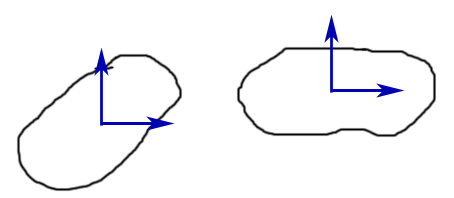
\includegraphics[width=0.30\textwidth]{articulatedbodies/softArt_G1.png}
	\caption{two bones}
	\label{2 Bones}
\end{figure}


Each of these bones contains several articulations points, also defined by rigids to have orientation information. \textsl{cf fig. 2}
\begin{figure}[htpb]
	\centering
		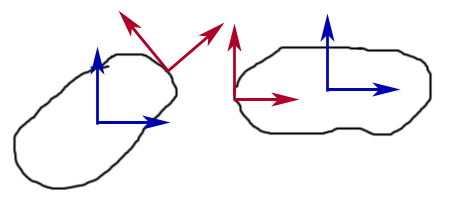
\includegraphics[width=0.30\textwidth]{articulatedbodies/softArt_G2.png}
	\caption{two bones (blue) with their articulation frames (red)}
\end{figure}

As seen previously, a joint between 2 bones is modeled by a 6-DOF spring. These springs are attached on the articulations points.    \textsl{cf fig. 3}
\begin{figure}[htpb]
	\centering
		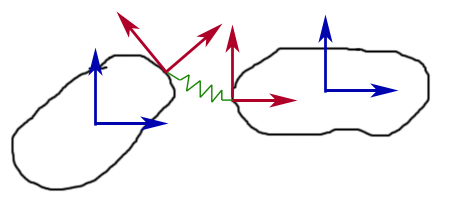
\includegraphics[width=0.30\textwidth]{articulatedbodies/softArt_G3.png}
	\caption{two bones linked by a joint-spring}
\end{figure}



\subsection{Sofa implementation}

To simulate these components in Sofa, we first need 2 mechanical objects : one for the bones (independent DOFs), and an other for the articulation points (mapped DOFs).
Each of them contains a list of rigid DOFs (respectively all the bones and all the articulations of the articulated body).
A mapping performs the link between the two lists, to know which articulations belong to which bones.


\subsubsection{Corresponding scene graph}
\begin{figure}[htpb]
	\centering
		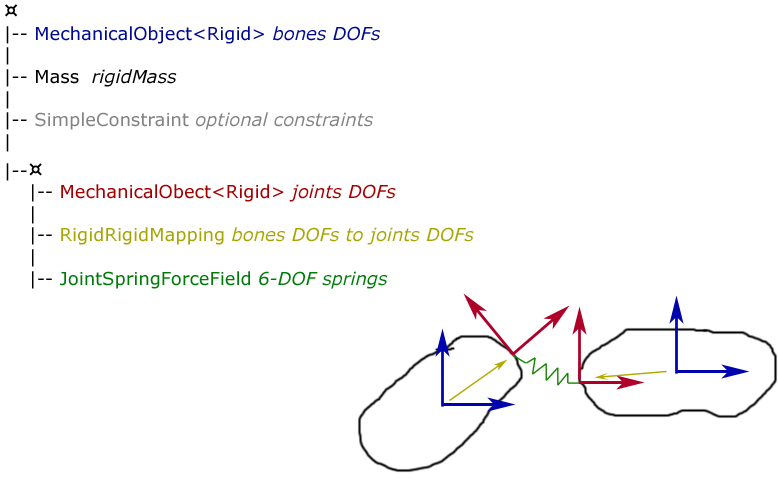
\includegraphics[width=0.90\textwidth]{articulatedbodies/scene_graph.png}
	\caption{a simple articulated body scene}
\end{figure}

\subsubsection {Example}

The example \texttt{../examples/Components/forcefield/JointSpringForceField.scn} shows a basic pendulum :

\begin{verbatim}
<Node>
  <Object type="BruteForceDetection"/>
  <Object type="DefaultContactManager"/>
  <Object type="DefaultPipeline"/>
  <Object type="ProximityIntersection"/>

  <Node>
    <Object type="CGImplicitSolver"	/>
    <Object type="MechanicalObject" template="Rigid" name="bones DOFs"
            position="0 0 0  0 0 0 1 
                      1 0 0  0 0 0 1 
                      3 0 0  0 0 0 1 
                      5 0 0  0 0 0 1 
                      7 0 0  0 0 0 1" />
    <Object type="UniformMass" template="Rigid" name="bones mass"
            mass="1 1 [1 0 0,0 1 0,0 0 1]" />
    <Object type="FixedConstraint" template="Rigid" name="fixOrigin"
            indices="0" />
		
    <Node>
      <Object type="MechanicalObject" template="Rigid" name="articulation points"
              position="0 0 0  0.707914 0 0 0.707914 
                       -1 0 0  0.707914 0 0 0.707914 
                        1 0 0  0.707914 0 0 0.707914 
                       -1 0 0  0.707914 0 0 0.707914 
                        1 0 0  0.707914 0 0 0.707914 
                       -1 0 0  0.707914 0 0 0.707914 
                        1 0 0  0.707914 0 0 0.707914 
                       -1 0 0  0.707914 0 0 0.707914 
                        1 0 0  0.707914 0 0 0.707914" />
      <Object type="RigidRigidMapping"
              repartition="1 2 2 2 2" />
      <Object type="JointSpringForceField" template="Rigid" name="joint springs"
              spring="BEGIN_SPRING 0 1  FREE_AXIS 0 0 0 0 1 0  ......  END_SPRING 
                      BEGIN_SPRING 2 3  FREE_AXIS 0 0 0 0 1 0  ......  END_SPRING 
                      BEGIN_SPRING 4 5  FREE_AXIS 0 0 0 0 1 0  ......  END_SPRING 
                      BEGIN_SPRING 6 7  FREE_AXIS 0 0 0 0 1 0  ......  END_SPRING " />
    </Node>
    <Node>
      <Object type="MechanicalObject" template="Vec3d"
              position="-1 -0.5 -0.5  -1 0.5 -0.5 ..." />
      <Object type="MeshTopology"
              lines="0 1  1 2  ..."
              triangles="3 1 0  3 2 1  ..." />
      <Object type="TriangleModel"/>
      <Object type="LineModel"/>
      <Object type="RigidMapping"
              repartition="0 8 8 8 8" />
    </Node>
  </Node>
</Node>

\end{verbatim}

\begin{figure}[htpb]
	\centering
		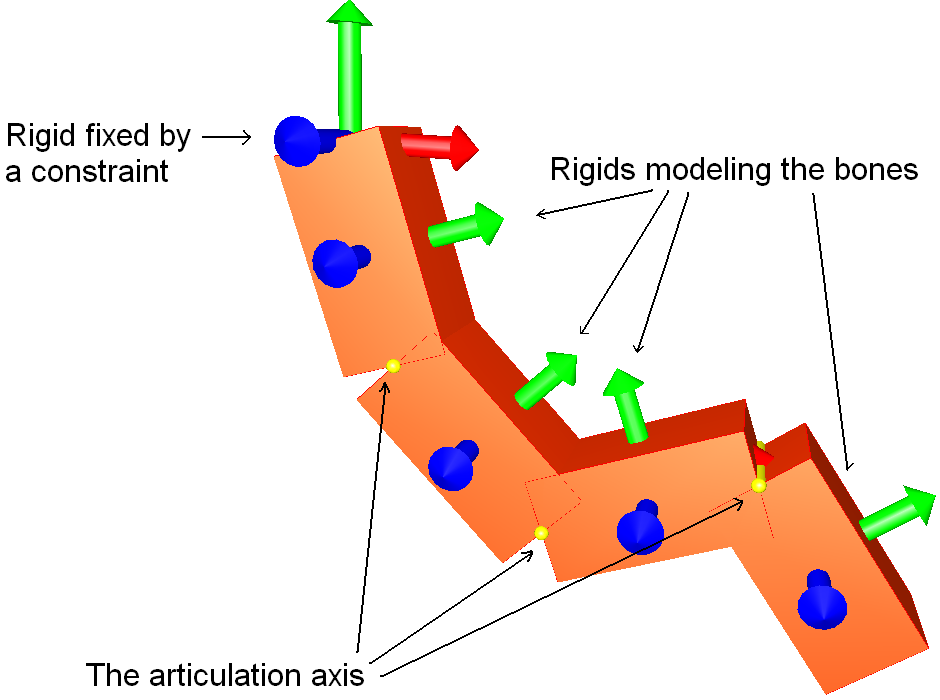
\includegraphics[width=0.70\textwidth]{articulatedbodies/softArt_snapshot.png}
	\caption{The pendulum is composed by 4 rigids linked one by one by articulations}
\end{figure}

In this example, we have under the first node the components to manage collisions, as usual.
Under the second node, we have :
\begin{itemize}
	\item the solver,
	\item the mechanical object modeling the independent rigid DOFs (5 rigids here),
	\item the rigid mass,
	\item a constraint, to fix the first rigid.
\end{itemize}

The third node (a child of the previous one) contains the components relative to the articulations :
\begin{itemize}
	\item the mechanical object modeling articulation points. Positions and orientations are relative to their parents.
	\item the mapping to link the two mechanical objects, as explained before. To know which articulations belong to which bones, a repartition vector is used. Several cases for this vector are possible :
		\begin{itemize}
			\item no value specified : every articulations belong to the first bone (classic rigid mapping).
			\item one value specified (ex: repartition="2") : each bone has the same number of articulations.
			\item number of bones values (like here, repartition="1 2 2 2 2") : the number of articulations is specified for each bone. For instance, here the first bone has 1 articulation, the next has 2 articulations, the next 2, Etc.
		\end{itemize}
	\item the JointSpringForceField containing the springs (4 springs here). Each spring is defined by a list of parameters, separated by tag names. Each spring is defined between the tags BEGIN\_SPRING and END\_SPRING. For instance here we have : "BEGIN\_SPRING 0 1  FREE\_AXIS 0 0 0 0 1 0  KS\_T 0.0 30000.0  KS\_R 0.0 200000.0  KS\_B 2000.0  KD 1.0  R\_LIM\_X -0.80 0.80  R\_LIM\_Y -1.57 1.57  R\_LIM\_Z 0.0 0.0  END\_SPRING".
		\begin{itemize}
			\item "0 1" are the indices of the two articulations the spring is attached to. They are the only compulsory parameters, the others are optional and take a default value if they are not specified.
			\item "FREE\_AXIS 0 0 0 0 1 0" design the free axis for the movements. it contains 6 booleans, one for each axis."0 0 0" mean that the 3 translation axis are constrained, and "0 1 0" mean that only the Y rotation axis is free.
			\item "KS\_T 0.0 30000.0" specify the stiffnesses to apply respectively for free translations and constrained translations.
			\item "KS\_R 0.0 200000.0" specify the stiffnesses to apply respectively for free rotations and constrained rotations.
			\item "KS\_B 2000.0" specify the stiffnesses to apply when an articulation is blocked, i.e. when a rotation exceeds the limit angle put on one axis.
			\item "KD 1.0" is the damping factor
			\item "R\_LIM\_X -0.80 0.80" design the limit angles (min and  max) on the x axis.
			\item "R\_LIM\_Y -1.57 1.57" design the limit angles (min and  max) on the y axis.
			\item "R\_LIM\_Z  0.0  0.0" design the limit angles (min and  max) on the z axis.
			\item It is also possible to specify "REST\_T x y z" and "REST\_R x y z t", which design the initial translation and rotation of the spring (in rest state).
		\end{itemize}
\end{itemize}

The last node contains the collision model. Nothing special here.


\subsection{Skinning}

The articulated body described previously models the skeleton of an object.
To have the external model (for the visual model or the collision model), which follows correctly the skeleton movements, it has to be mapped with the skeleton. 
\ 
A skinning mapping allows us to do this link. The external model is from this moment to deform itself smoothly, i.e. without breaking points around the articulations.

The influence of the bones on each point of the external model is given by skinning weights.
2 ways are possible to set the skinning weights to the mapping :
\begin{itemize}
	\item Either the user gives directly the weights list to the mapping. It is useful if good weights have been pre computed previsouly, like in Maya for instance.
	\item Else, the user defines a number of references \textsl{n} that will be used for mapped points. Then, each external model point will search its \textsl{n} nearest bones (mechanical DOFs), and then compute the skinning weights from the relation :
\[ W = \frac{1}{d^{2}}  \]
\small{ with \textsl{d} : the distance between the external point and the rigid DOF.}
\end{itemize}

\begin{figure*}[htpb]
		\centering
		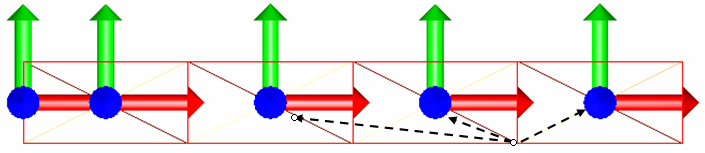
\includegraphics[width=0.50\textwidth]{articulatedbodies/skinning}
		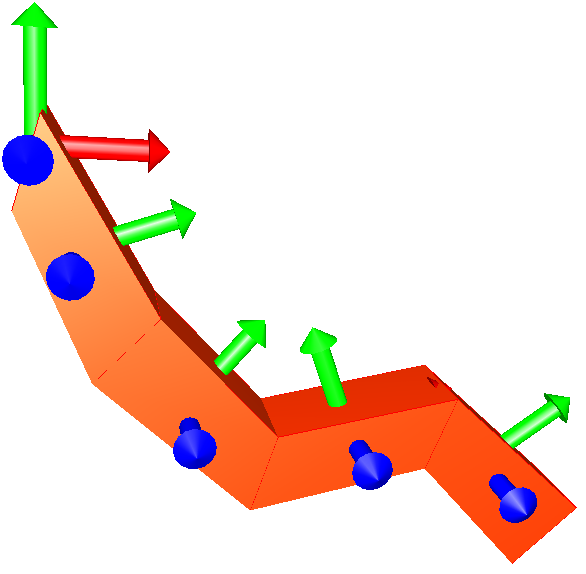
\includegraphics[width=0.30\textwidth]{articulatedbodies/skinnedPendulum}	
	\caption{In the example \texttt{../examples/Components/mapping/SkinningMapping.scn} the external points compute their skinning weights from the 3 nearest DOFs}
\end{figure*}

\begin{figure*}[htpb]
		\centering
		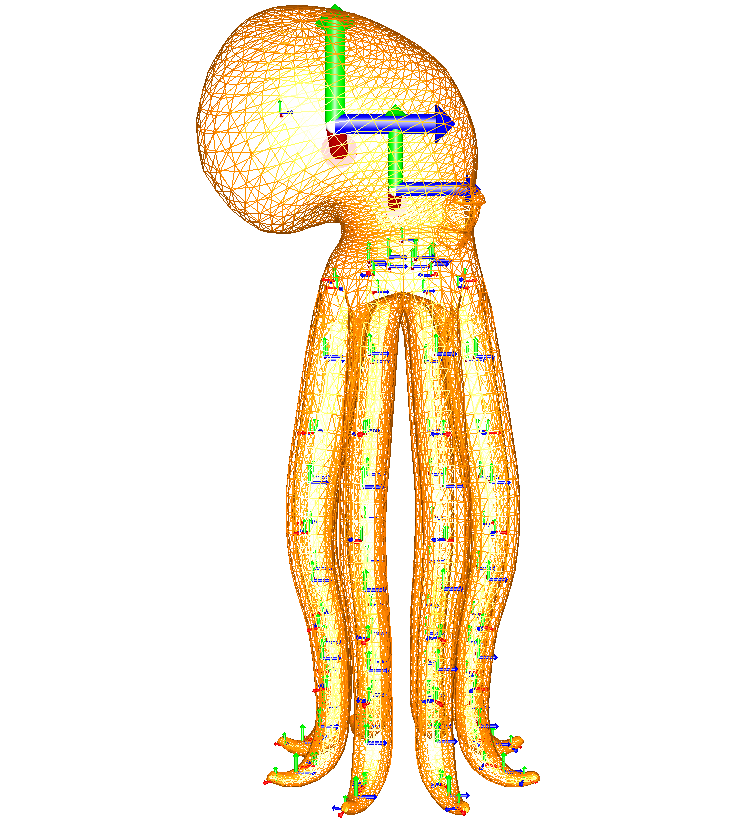
\includegraphics[width=0.40\textwidth]{articulatedbodies/teodule_wireframe}	
		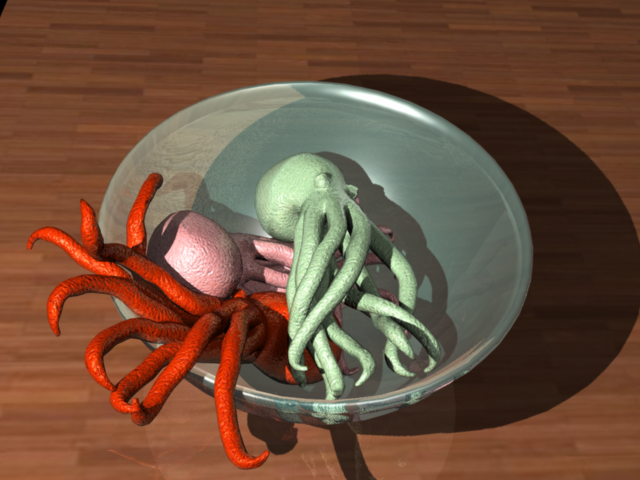
\includegraphics[width=0.50\textwidth]{articulatedbodies/teodule_soupedepoulpe}	
	\caption{soft articulations coupled with skinning allow complexe model deformations}
\end{figure*}

\newpage
\section{How to use mesh topologies in SOFA}

H. Delingette, B. Andr�

\subsection{Introduction}

While mesh geometry describes where mesh vertices are located in space, mesh topology tells 
how vertices are connected to each other by edges, triangles or any type of mesh element. 
Both information are required on a computational mesh to perform :

\begin{itemize}

 \item \textbf{Mesh Visualization},

 \item \textbf{Collision detection} : some collision detection are mesh based (e.g.
triangles or edges),

 \item \textbf{Mechanical Modeling} : deforming a mesh also requires to the
knowledge of a mesh topology. For instance a spring mass model
requires knowing about the edges that connects pair of vertices,

 \item \textbf{Haptic rendering},

 \item \textbf{Description of scalar} (temperature, electric potential, etc.) or
vectorial fields (speed, fiber orientation, etc.)

\end{itemize}

Since topological changes are essential for surgery simulators, a common difficulty when designing those simulators is to ensure that the visual, mechanical, haptic and collision behavior of all meshes stay valid and consistent upon any topological change. 

Our approach to  handle topological changes is modular since each software component (collision detection, mechanical solver$\ldots$) may be written with little knowledge about the nature of other components. It is versatile because any type of topological changes can be handled with the proposed design. 

Our objective to keep a modular design implies that mesh related information (such as mechanical or visual properties) is not centralized in the mesh data structure but is stored in the software components that are using this information. Furthermore, we manage an efficient and direct storage of information into arrays despite the renumbering of elements that occur during topological changes.

\subsection{Family of Topologies} 


We focus the topology description on meshes that are cellular complexes made of $k$-simplices (triangulations, tetrahedralisation) or $k$-cubes (quad or hexahedron meshes). These meshes are the most commonly used in real-time surgery simulation and can be hierarchically decomposed into $k$-cells, edges being $1$-cells, triangles and quads being $2$-cells, tetrahedron and hexahedron being $3$-cells. 
To take advantage of this feature, the  different mesh topologies are structured as a family tree (see Fig.~\ref{fig:BW_Topology_Family_Tree}) where children topologies are made of their parent topology. This hierarchy makes the design of simulation components very versatile since a component working on a given mesh topology type will also work on derived types. For instance a spring-mass mechanical component only requires the knowledge of a list of edges (an {\em Edge Set Topology} as described in Fig.~\ref{fig:BW_Topology_Family_Tree}) to be effective. With the proposed design, this component can be used with no changes on triangulation or hexahedral meshes.
 
The proposed hierarchy makes also a distinction between conformal and manifold meshes. While most common FEM components require a mesh to be conformal (but not necessarily manifold), many high-level software components (such as cutting, contact, haptic feedback algorithms) require the mesh to be a manifold where a surface normal is well-defined at each vertex.   


\begin{figure}[ht]
    \centering
        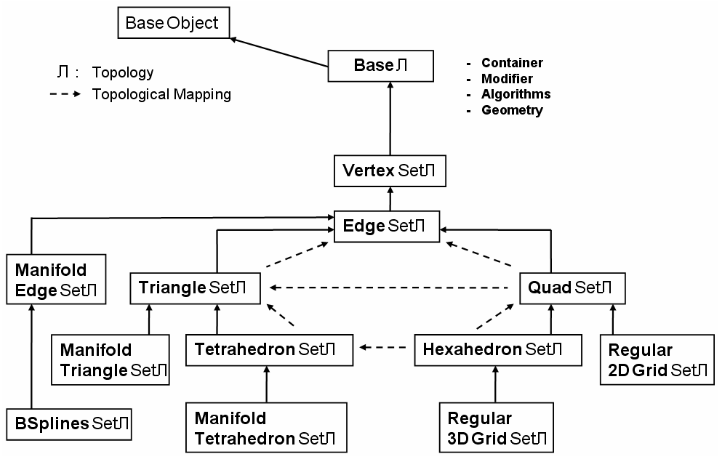
\includegraphics[width=0.85\textwidth]{topology/BW_Topology_Family_Tree.png}
     \caption{Family tree of topology objects. Dashed arrows indicate possible {\em Topological Mappings} from a topology object to another.}
    \label{fig:BW_Topology_Family_Tree}
\end{figure}

Topology objects are composed of four functional members:{\em Container}, {\em Modifier}, {\em Algorithms} and {\em Geometry}.

\begin{itemize}

 \item The {\em Container} member creates and updates when needed two complementary arrays (see Fig.~\ref{fig:BW_Sub_Shell_Diagram}). The former describes the $l$-cells included in a single $k$-cell, $l<k$, while the latter gives the $k$-cells adjacent to a single $l$-cell.
 
 \item The {\em Modifier} member provides low-level methods that implement elementary topological changes such as the removal or addition of an element. 
 
 \item The {\em Algorithms} member provides high-level topological modification methods (cutting, refinement) which decompose complex tasks into low-level ones). 
 
 \item The {\em Geometry} member provides geometrical information about the mesh ({\em e.g.} length, normal, curvature, ...) and requires the knowledge of the vertex positions stored in the {\em Degrees of Freedom} component. 
 
\end{itemize}


\begin{figure}[ht]
    \centering
        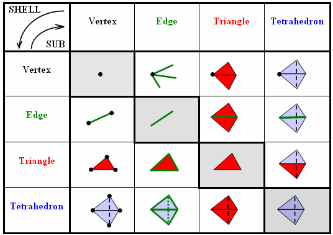
\includegraphics[width=0.6\textwidth]{topology/Sub_Shell_Diagram}
    \caption{The two topological arrays stored in a {\em Container} correspond to the upper and lower triangular entries of this table. The upper entries provide the $k$-cells adjacent to a $l$-cell, $l<k$. The lower entries describe the $l$-cells included in a $k$-cell. Similar table exists for quad and hexahedron elements.}
    \label{fig:BW_Sub_Shell_Diagram}
\end{figure}

\subsection{Component-Related Data Structure}

A key feature of our design is that containers storing mesh information (material stiffness, list of fixed vertices, nodal masses, ...) are stored in {\em components} and spread out in the simulation tree. This modular approach is in sharp contrast with a centralized storage of information in the mesh data structure through the use of generic pointers or template classes.  

Another choice is that most containers are simple arrays with contiguous memory storage and a short direct access time.
This is important for real-time simulation, but bears some drawbacks when elements of these arrays are being removed since it entails the renumbering of elements. For instance, when a single element is removed, the last array element is renumbered such that the array stays contiguous. Fortunately, all renumbering tasks that maintain consistent arrays can be automated and hidden to the user when topological changes in the mesh arise.
Besides, time to update data structures does not depends on the total number of mesh elements but only on the number of modified elements.
Therefore, in our framework, mesh data structures are stored in simple and efficient containers, the complexity of keeping the container consistent with topological changes being automated.

There are as many containers as topological elements: vertices, edges, triangles, ... . These containers are similar to the STL {\em std::vector} classes and allow one to store any component-related data structure. A typical implementation of spring-mass models would use an edge container that stores for each edge, the spring stiffness and damping value, the $i^{th}$ element of that container being implicitly associated with the $i^{th}$ edge of the topology. Finally, two other types of containers may be used when needed. The former stores a data structure for a subset of topological elements (for instance pressure on surface triangles in a tetrahedralisation) while the latter stores only a subset of element indices.


\subsection{Handling Topological Changes}

\noindent 
Surgery simulation involves complex topological changes on meshes, 
for example when cutting a surface along a line segment, or when locally refining a volume before removing some tissue.
However, one can always decompose these complex changes into a sequence of elementary operations, 
such as adding an element, removing an element, renumbering a list of elements or modifying a vertex position.

Our approach to handle topological changes makes the update of data structures transparent to the user, through a mechanism of propagation of topological events.
A topological event corresponds to the intent to add or to
remove a list of topological elements. But the removal of elements cannot be tackled in the same way as the addition of elements. Indeed, the element removal event must be first notified to
the other components before the element is actually removed by the {\em Modifier}.
Conversely, element addition is first processed by the {\em Modifier} and then element addition event is notified to other components (see Fig.~\ref{fig:Order_Notifications}).
Besides, the events notifying the creation of elements also include a list of ancestor elements. Therefore, when splitting one triangle into two sub-triangles (see Fig.~\ref{fig:7_Steps_Cutting_Algorithm}), each component-related information ({\em e.g.} its Young modulus or its mass density) associated with a sub-triangle will be created knowing that the sub-triangle originates from a specific triangle. Such mechanism is important to deal with meshes with non-homogeneous characteristics related to the presence of pathologies.

\begin{figure}[ht]
    \centering
        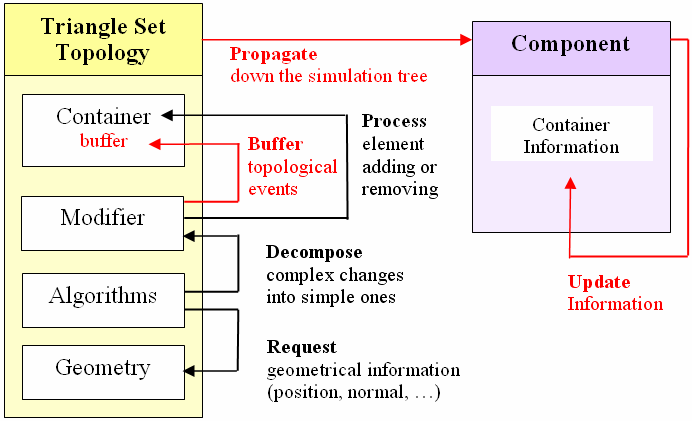
\includegraphics[width=0.7\textwidth]{topology/Handling_Changes}
    \caption{Handling topological changes, with the example of a {\em Triangle Set Topology}. 
    {\em Component} corresponds to any component of the simulation which may need topological information to perform a specific task.
    Black features indicate the effective change process. Red features show the steps of event notification.}
    \label{fig:Handling_Changes}
\end{figure}

\begin{figure}[ht]
 \centering
 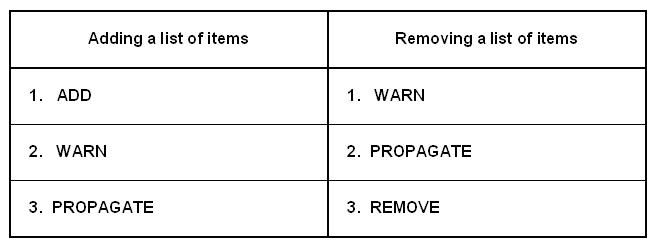
\includegraphics[width=0.65\linewidth]{topology/Order_Notifications}
  \caption{Order to respect when adding or removing an item. WARN means : add the current topological change (add or delete a list of items) in the list of TopologyChanges. PROPAGATE means :  traverse the simulation tree with a TopologyChangeVistor to send the current topological change event to all force fields, constraints, mappings, etc.}
 \label{fig:Order_Notifications}
\end{figure}


\begin{figure}[ht]
    \centering
        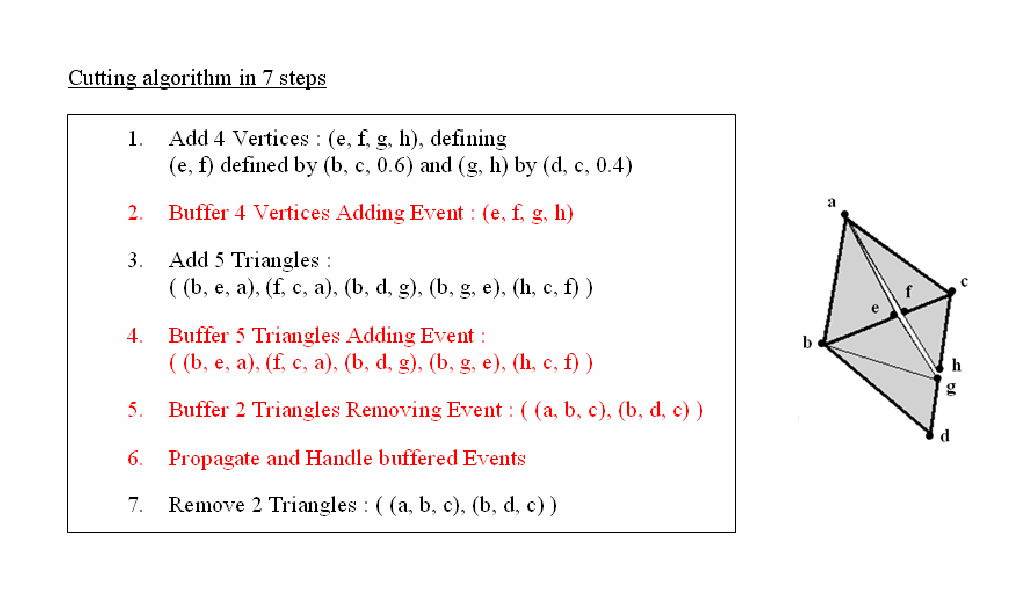
\includegraphics[width=0.8\textwidth]{topology/7_Steps_Cutting_Algorithm}
    \caption{Seven steps to perform cutting along two triangles (these generic steps would be the same to cut an arbitrarily number of triangles).
    Black steps indicate the effective change process. Red steps show the steps of event notification.}
    \label{fig:7_Steps_Cutting_Algorithm}
\end{figure}


The mechanism to handle topological changes is illustrated by Fig.~\ref{fig:Handling_Changes}.
The notification step consists in accumulating the sequence of
topological events  involved in a high-level topological change into a buffer stored in
the {\em Container}. Then the event list is propagated to all its
neighbors and leaves beneath by using a visitor mechanism, called a
{\em Topology Visitor}. Once a given component is visited, the topological
events are actually processed one by one and the data structure used to store mesh related information are automatically updated.

In practice, for each specific component ({\em e.g.} spring-mass mechanical component), a set of callback functions are provided describing how to update the data structure ({\em e.g.} spring stiffness and damping values) when adding or removing an element ({\em e.g.} the edges defined by the two extremities of the springs).
We applied the observer design pattern so that component-related data structures update themselves automatically.


\subsection{Combining Topologies}

Handling a single mesh topology in a surgery simulation scene is often too restrictive. There are at least three common situations where it is necessary to have, for the same mesh, several topological descriptions sharing the same degrees of freedom: the {\em boundary}, {\em composite} and {\em surrogate} cases. In the {\em boundary } scenario,  specific  
algorithms may be applied to the boundary of a mesh, the boundary of tetrahedral mesh being a triangulated mesh and that of a triangular mesh being a polygonal line. For instance, those algorithms may consist of applying additional membrane forces ({\em e.g.} to simulate the effect of the Glisson capsule in the liver) or visualizing a textured surface. Rather than designing specific simulation components to handle triangulations as the border of tetrahedrisations, our  framework allows us to create a triangulation topology object from  a tetrahedrisation mesh and to use regular components associated with triangulations.

The {\em composite} scenario consists in having a mesh that includes several types of elements: triangles with quads, or hexahedra with tetrahedra. Instead of designing specific components for those composite meshes, it is simpler and more versatile to reuse components that are dedicated to each mesh type. Finally the {\em surrogate} scenario corresponds to cases where one topological element may be replaced by a set of elements of a different type with the same degrees of freedom. For instance a quad may be split into two triangles while an hexahedron may be split into several tetrahedra. Thus a quad mesh may also be viewed as a triangular mesh whose topology is constrained by the quad mesh topology.

\begin{figure}[ht]
    \centering
        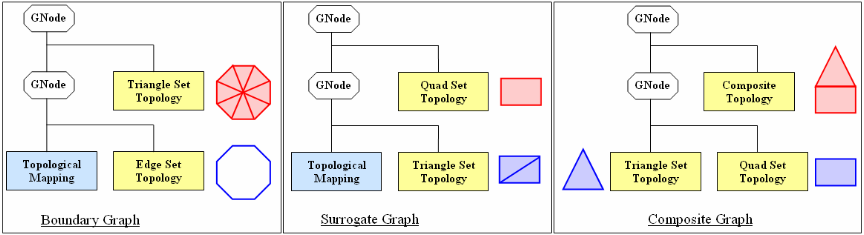
\includegraphics[width=1.0\textwidth]{topology/Combining_Topologies}
    \caption{Three scenari examples to combine topologies. ({\em From left to right}) A {\em Boundary Graph} from a triangle set to an edge set, a {\em Surrogate Graph} from a quad set to an triangle set and a {\em Composite Graph} superseding a quad set and a triangle set.}
    \label{fig:Combining_Topologies}
\end{figure}

These three cases can be handled seamlessly by using a graph of multiple topologies, the topology object being at the top node having the specific role of controlling the topologies below. Although we chose to duplicate topological information in memory, it has no effect on the time required to compute the forces.  Fig.~\ref{fig:Scene_Graph_TopologicalMapping} provides an example of a border scenario (triangulation as the border of a tetrahedralisation) while Fig.~\ref{fig:Combining_Topologies} shows general layout of topology graphs in the three cases described previously. In any cases, those graphs include a dedicated component called a {\em Topological Mapping} whose objectives are twofold. First, they translate topological events originating from the master topology ({\em e.g.} remove this quad) into topological actions suitable for the slave topology ({\em e.g} remove those two triangles for a surrogate scenario). Second, they provide index equivalence  between global numbering of elements in the master topology ({\em e.g} a triangle index in a tetrahedralisation topology ) and local numbering in the slave topology ({\em e.g} the index of the same triangle in the border triangulation). Possible {\em Topological Mappings} from a topology object to another have been represented by blue arrows in Fig.~\ref{fig:BW_Topology_Family_Tree}.

Note that those topology graphs can be combined and cascaded, for instance by constructing the triangulation border of a tetrahedrisation created from an hexahedral mesh.  But only topology algorithms of the master topology may be called to simulate cutting or to locally refine a volume. By combining topology graphs with generic components one can simulate fairly complex simulation scenes where topological changes can be seamlessly applied.


\subsection{An example of Topological Mapping : from TetrahedronSetTopology to TriangleSetTopology}

A TopologicalMapping is a new kind of Mapping which converts an
input topology to an output topology (both topologies are of type
BaseTopology).
\\

It first initializes the mesh of the output topology from the mesh
of the input topology, and it creates the two Index Maps that
maintain the correspondence between the indices of their common
elements.
\\

Then, at each propagation of topological changes, it translates the
topological change events that are propagated from the input
topology into specific actions that call element adding methods or
element removal methods on the output topology, and it updates the
Index Maps.
\\

So, at each time step, the geometrical and adjacency information are
consistent in both topologies.

Here is the scene-graph corresponding to the simulation of an object
which can be represented as a tetrahedral volume (on which one
volume force is applied) or as a triangular surface (on which two
surface forces are applied). Note that the Visual Model and the
Collsion Model are attached to the surface mesh of the object :


\begin{figure}[ht]
 \centering
 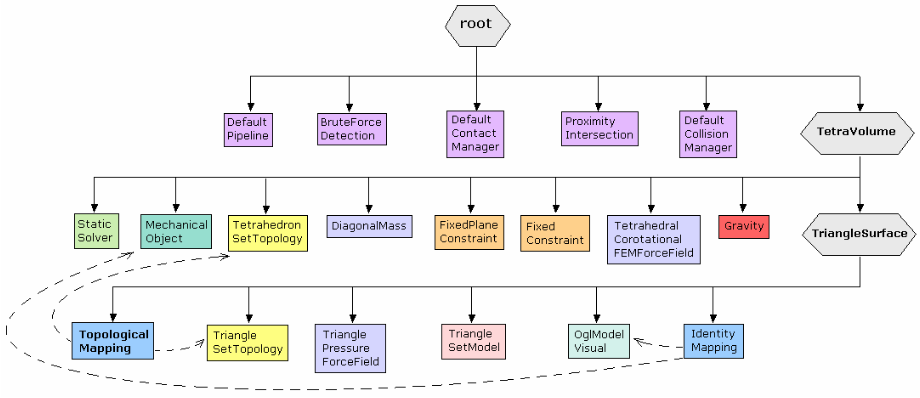
\includegraphics[width=1.0\linewidth]{topology/Scene_Graph_TopologicalMapping}
  \caption{Scene Graph illustrating a TopologicalMapping from a TetrahedronSetTopology to a TriangleSetTopology.}
 \label{fig:Scene_Graph_TopologicalMapping}
\end{figure}

Let us consider an example where the user wants to remove one tetraheron (whose one triangle at least is visible) from the tetrahedral volume.
The component Tetra$2$TriangleSetTopology handles this topological change by following five steps :
\\


\begin{itemize}

    \item \textbf{Step $1$.} The user right-clicks on visible triangle T in the scene, which is detected by the Collision Model and indexed by $loc\_T$ in the triangular surface mesh.
    
\begin{figure*}
 \centering
 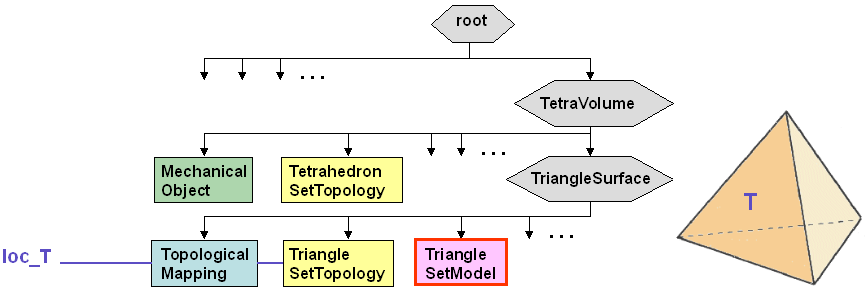
\includegraphics[width=1.0\linewidth]{topology/TopoMap_example_1}
  \caption{Scenario when the user wants to remove one tetraheron.- Step 1.}
 \label{fig:TopoMap_example_1}
\end{figure*}


    \item \textbf{Step $2$.} If a Topological Mapping of type ( input = TetrahedronSetTopology, output = TriangleSetTopology ) does exist, the index map $Loc2GlobVec$ is requested to give the index $glob\_T$ which is indexing the triangle T in the tetrahedral volume mesh. 
The TetrahedronTriangleShell gives then the index $ind\_TE$ which is indexing the unique tetrahedron TE containing T. 
We call the action RemoveTetrahedra($< ind\_TE >$) on the input topology.

\begin{figure*}
 \centering
 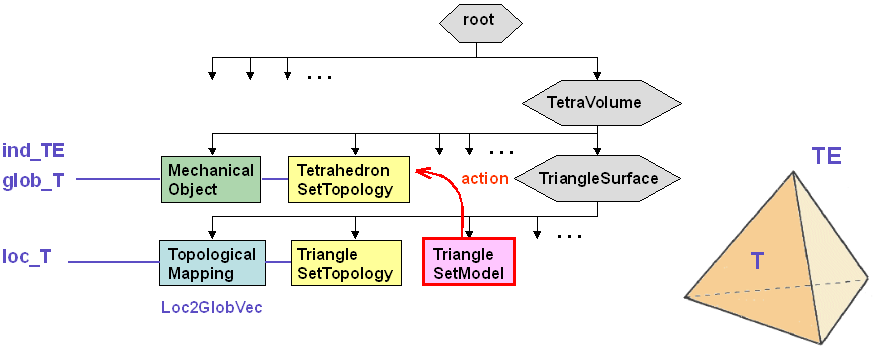
\includegraphics[width=1.0\linewidth]{topology/TopoMap_example_2}
  \caption{Scenario when the user wants to remove one tetraheron.- Step 2.}
 \label{fig:TopoMap_example_2}
\end{figure*}


    \item \textbf{Step $3$}. The TetrahedronSetTopology notifies all the removal events, that are successively concerning one tetrahedron, one or more isolated triangles, the possibly isolated edges and the possibly isolated points.

\begin{figure*}
 \centering
 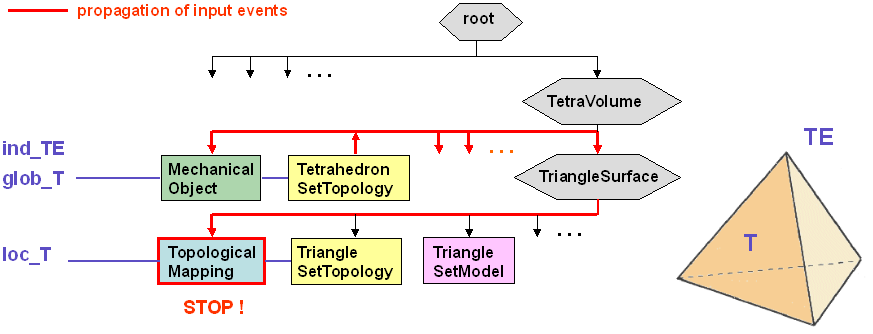
\includegraphics[width=1.0\linewidth]{topology/TopoMap_example_3}
  \caption{Scenario when the user wants to remove one tetraheron.- Step 3.}
 \label{fig:TopoMap_example_3}
\end{figure*}


    \item \textbf{Step $4$.} The propagation of topological events reaches a Topological Mapping which is strictly lower in the scene graph, then it stops.
The Tetra2TriangleTopologicalMapping translates the input events into output actions on the TriangleSetTopology.
The event Tetrahedron removal is translated into the action AddTriangles ( $<$ indices of new visible triangles $>$ ).
The event Triangle removal is translated into the action RemoveTriangles ( $<$ indices of destroyed triangles $>$, removeDOF $=$ false ), where (removeDOF $=$ false) indicates that the DOFs of the isolated points must not be deleted because they have already been removed by the input topology.
The Index maps ( Loc2GlobVec, Glob2LocMap, In2OutMap ) are requested and updated to maintain the correspondence between the items indices in input and output topologies.

\begin{figure*}
 \centering
 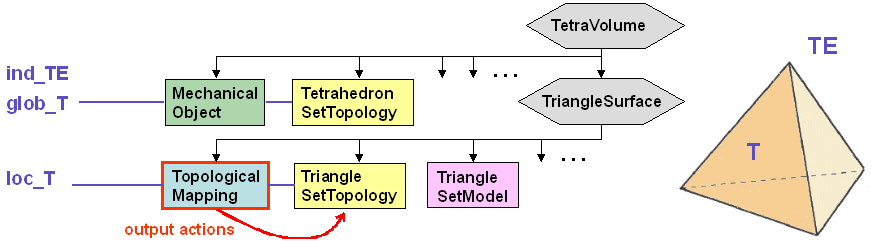
\includegraphics[width=1.0\linewidth]{topology/TopoMap_example_4}
  \caption{Scenario when the user wants to remove one tetraheron.- Step 4.}
 \label{fig:TopoMap_example_4}
\end{figure*}


    \item \textbf{Step $5$.} The adding events concerning one or more new visible triangles and the removal events concerning one or more isolated triangles are notified from the TriangleSetTopology.

\begin{figure*}
 \centering
 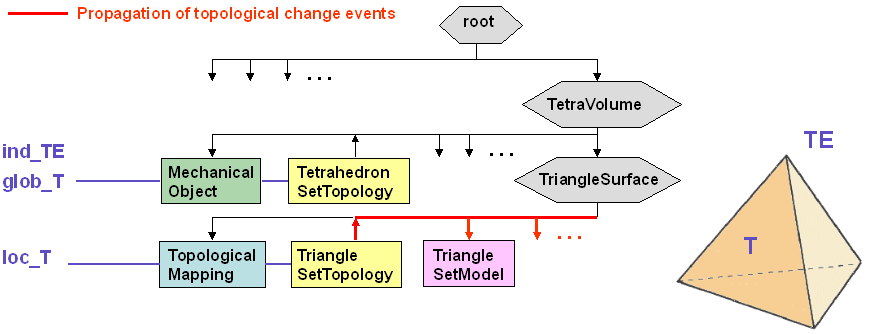
\includegraphics[width=1.0\linewidth]{topology/TopoMap_example_5}
  \caption{Scenario when the user wants to remove one tetraheron.- Step 5.}
 \label{fig:TopoMap_example_5}
\end{figure*}

\end{itemize}

\subsection{Example of scene file with a topological mapping}

\begin{figure*}
 \centering
 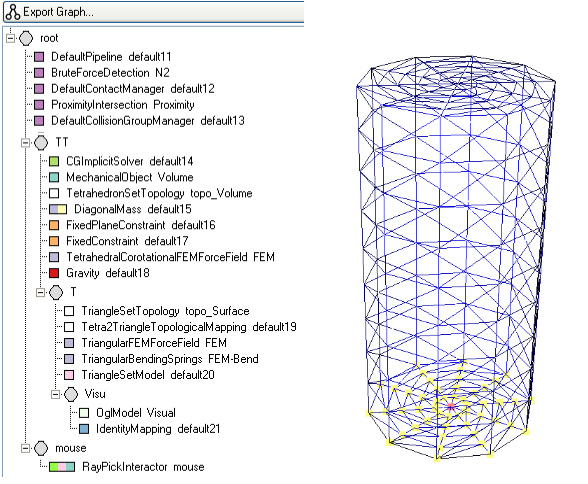
\includegraphics[width=0.9\linewidth]{topology/cylinder_example}
  \caption{Scene Graph simulating a bending cylinder as a tetrahedral volume and as a triangular surface (the cylinder membrane)}
 \label{fig:cylinder_example}
\end{figure*}

\newpage

Here is the scene file corresponding to the example :

\begin{verbatim}

<Node name="root" dt="0.05" showBehaviorModels="1" showCollisionModels="0" showMappings="0" 
 showForceFields="0" showBoundingTree="0" gravity="0 0 0">
  
	<Object type="CollisionPipeline" verbose="0" />
	<Object type="BruteForceDetection" name="N2" />
	<Object type="CollisionResponse" response="default" />
	<Object type="MinProximityIntersection" name="Proximity" alarmDistance="0.8" 
	 contactDistance="0.5" />
	
	<Object type="CollisionGroup" />

	<Node name="TT">
	
		<Object type="EulerImplicit" name="cg_odesolver" printLog="false"/>
		<Object type="CGLinearSolver" iterations="25" name="linear solver" tolerance="1.0e-9" 
		 threshold="1.0e-9" />
		
		<Object type="MeshLoader" name="meshLoader" filename="mesh/cylinder.msh" />
		<Object type="MechanicalObject" name="Volume" />
		<include href="Objects/TetrahedronSetTopology.xml" />

    <Object type="DiagonalMass" massDensity="0.5" />
		<Object type="FixedPlaneConstraint" direction="0 0 1" dmin="-0.1" dmax="0.1"/>
		<Object type="FixedConstraint" indices="0" />		
    <Object type="TetrahedralCorotationalFEMForceField" name="FEM" youngModulus="60" 
     poissonRatio="0.3" method="large" />
    
    <Object type="Gravity" gravity="0 0 0"/>

		<Node name="T">
		
			<include href="Objects/TriangleSetTopology.xml" />
			<Object type="Tetra2TriangleTopologicalMapping" object1="../../Container" object2="Container"/>

      <Object type="TriangularFEMForceField" name="FEM" youngModulus="10" poissonRatio="0.3" 
       method="large" /> 
			
			<Object type="TriangularBendingSprings" name="FEM-Bend" stiffness="300" damping="1.0"/>		
			    
			<Object type="TriangleSet"/>

			<Node name="Visu">
			
				<Object type="OglModel" name="Visual" color="blue" />
				<Object type="IdentityMapping" object1="../../../Volume" object2="Visual" />
				
			</Node>						
			
		</Node>
		
	</Node>
	
</Node>

\end{verbatim}

Here is the example of the included TriangleSetTopology.xml file, where the four members of the {\em TriangleSetTopology} are defined :

\begin{verbatim}

<Node name="Group"> 
  <Object type="TriangleSetTopologyContainer"  name="Container" />
  <Object type="TriangleSetTopologyModifier"   name="Modifier" />
  <Object type="TriangleSetTopologyAlgorithms" name="TopoAlgo"   template="Vec3d" />
  <Object type="TriangleSetGeometryAlgorithms" name="GeomAlgo"   template="Vec3d" />
</Node>

\end{verbatim}

\subsection{How to make a component aware of topological changes ?}

%%%

There are actually a few generic lines of code to add in a component for it to handle topological changes.
\\

If the component is based on topological elements like edges, the main idea is to introduce an object {\em edgeinfo} of type {\em EdgeData} 
and to template it by a data structure {\em EdgeInformation} that is attached to each edge (this data structure has to be defined by the component, to which it is specific).
By calling the method {\em handleTopologyEvents} on the object {\em edgeinfo} (of type {\em EdgeData} $<${\em EdgeInformation}$>$), the component-related data structure is automatically updated (code has been implement in file {\em EdgeData.inl}).
\\

Here : {\em edgeinfo}$[i]$ is the data structure attached to the edge indexed by $i$ in the topological component {\em EdgeSetTopology}.
\\

In SOFA, among the existing ForceField component able to handle topological changes there are for example : {\em BeamFEMForceField} (for the simple case) and {\em TriangularBendingSprings} (for the complicated case : data structure attached to each edge need to contain indices of points, which must also be updated by the method {\em handleTopologyChange}).
\\

For the simple case, here is how to adapt a Force Field component called {\em totoForceField} (for instance based on elements of type edge) to topological changes : 

\subsubsection{Modifications in header file {\em totoForceField.h} :}

\begin{itemize}

	\item Include the following header :  \begin{verbatim} #include <sofa/component/topology/EdgeData.h> \end{verbatim}
	
	\item Define a structure {\em EdgeInformation} which describes the information attached to each edge (for example {\em spring stiffness},
{\em spring length}, ...)
	
	\item Add an object {\em edgeinfo} of type {\em EdgeData} templated by the type
{\em EdgeInformation} : \begin{verbatim} topology::EdgeData<EdgeInformation> edgeinfo;  \end{verbatim}

	\item Declare the virtual method {\em handleTopologyChange} : \begin{verbatim} virtual void handleTopologyChange(); \end{verbatim}

  \item Add the callback function for the creation of edges :

\begin{verbatim} 

static void EdgeCreationFunction(
    int edgeIndex,
    void* param,
    EdgeInformation &ei,
    const topology::Edge& ,
    const sofa::helper::vector< unsigned int > &,
    const sofa::helper::vector< double >&
);


\end{verbatim} 

\end{itemize}

\subsubsection{Modifications in inline file {\em totoForceField.inl} :}


\begin{itemize}

	\item Add at the end of the method {\em init()} to specify the callbacks :
	
	\begin{verbatim} 

edgeinfo.setCreateFunction(EdgeCreationFunction);
edgeinfo.setCreateParameter( (void *) this );
edgeinfo.setDestroyParameter( (void *) this );

\end{verbatim} 
	
	\item Implement the method {\em handleTopologyChange()} :
	
  \begin{verbatim} 

template <class DataTypes>
void totoForceField<DataTypes>::handleTopologyChange()
{

    std::list< const sofa::core::componentmodel::topology::TopologyChange* >
::const_iterator itBegin = _topology->firstChange();

    std::list< const sofa::core::componentmodel::topology::TopologyChange*>
::const_iterator itEnd = _topology->lastChange();

    edgeinfo.handleTopologyEvents(itBegin,itEnd);
    
}
\end{verbatim} 

	\item Implement the method {\em EdgeCreationFunction} (usefull for the initialization of the data attacheed to a new edge) :
	
	\begin{verbatim} 
	
template<class DataTypes>
void totoForceField<DataTypes>::EdgeCreationFunction(

int edgeIndex, void* param, EdgeInformation &ei,
const topology::Edge& e,  const sofa::helper::vector< unsigned int > &a,
const sofa::helper::vector< double >&
)

{

    totoForceField<DataTypes> *ff= (totoForceField<DataTypes> *)param;

    if (ff) {

      ei.champ = value; // initialiser tous les champs de "edgeinfo[i]"

      (...)

    }
}
	
	\end{verbatim} 
	
	
\end{itemize}

At any time, it is possible to access the information from the container member of the topology (so as to get some neighborhood information) by using a pointer to the {\em BaseMeshTopology} API :

	\begin{verbatim} 
	
sofa::core::componentmodel::topology::BaseMeshTopology* _topology;
_topology = getContext()->getMeshTopology();

	\end{verbatim} 


\subsection{What happens when I split an Edge ?}

\begin{figure*}[htpb]
 \centering
 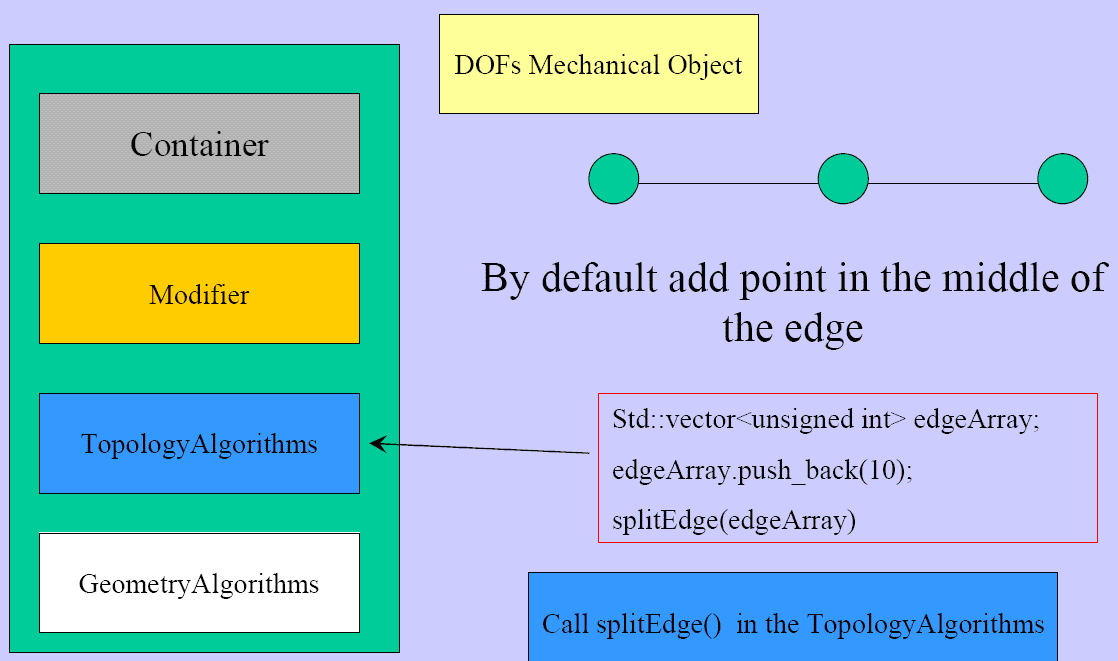
\includegraphics[width=0.9\linewidth]{topology/Topology_Example_1}
 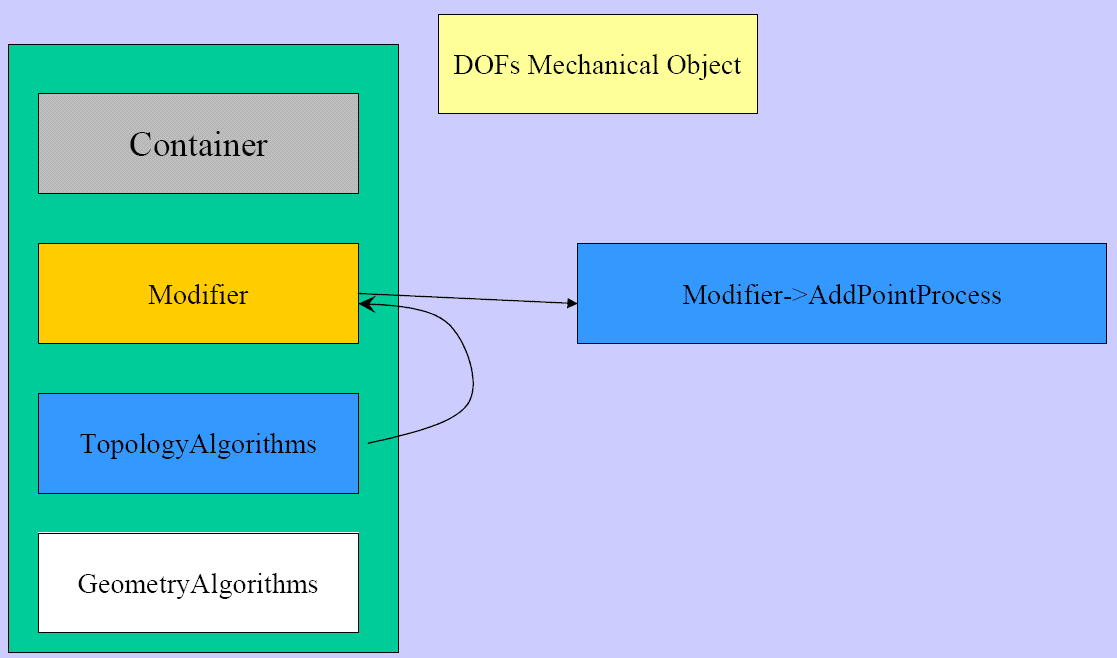
\includegraphics[width=0.9\linewidth]{topology/Topology_Example_2}
  \caption{What happens when I split an Edge ? - Step 1. 2.}
 \label{fig:Topology_Example_12}
\end{figure*}

\newpage

\begin{figure*}[htpb]
 \centering
 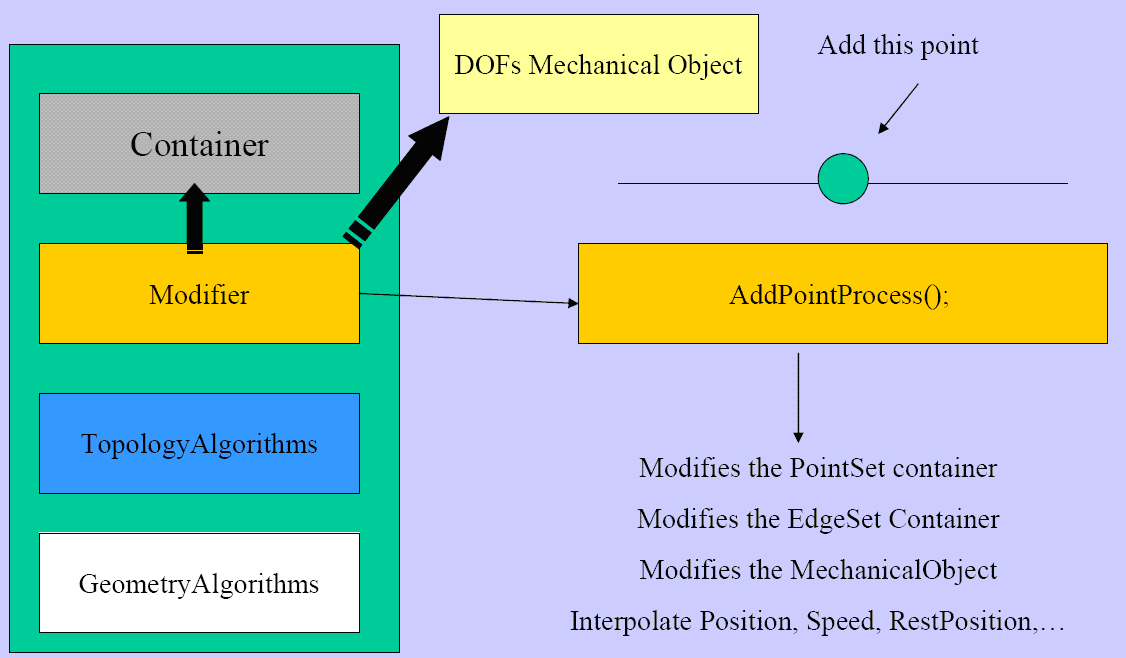
\includegraphics[width=0.9\linewidth]{topology/Topology_Example_3}
 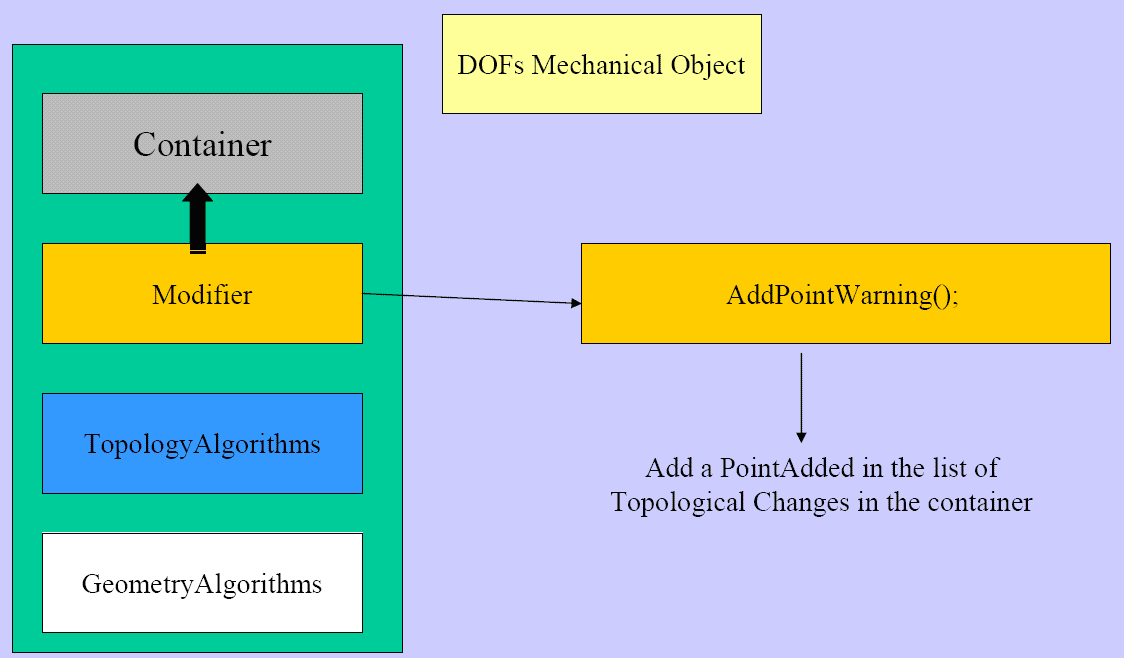
\includegraphics[width=0.9\linewidth]{topology/Topology_Example_4}
  \caption{What happens when I split an Edge ? - Step 3. 4.}
 \label{fig:Topology_Example_34}
\end{figure*}

\newpage

\begin{figure*}[htpb]
 \centering
 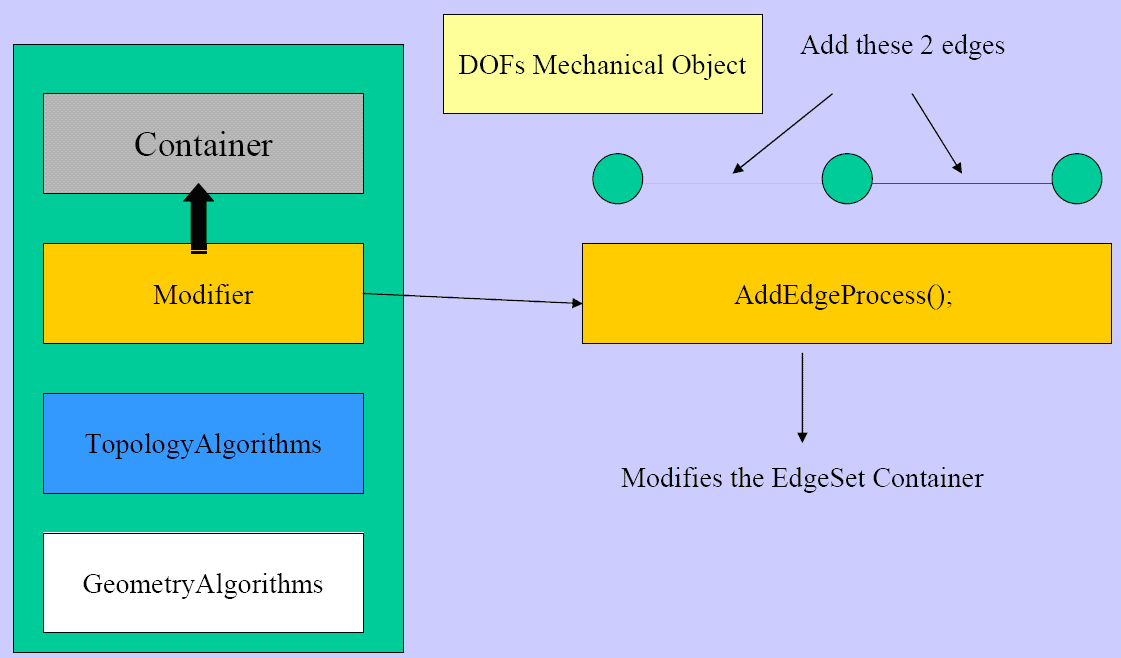
\includegraphics[width=0.9\linewidth]{topology/Topology_Example_5}
 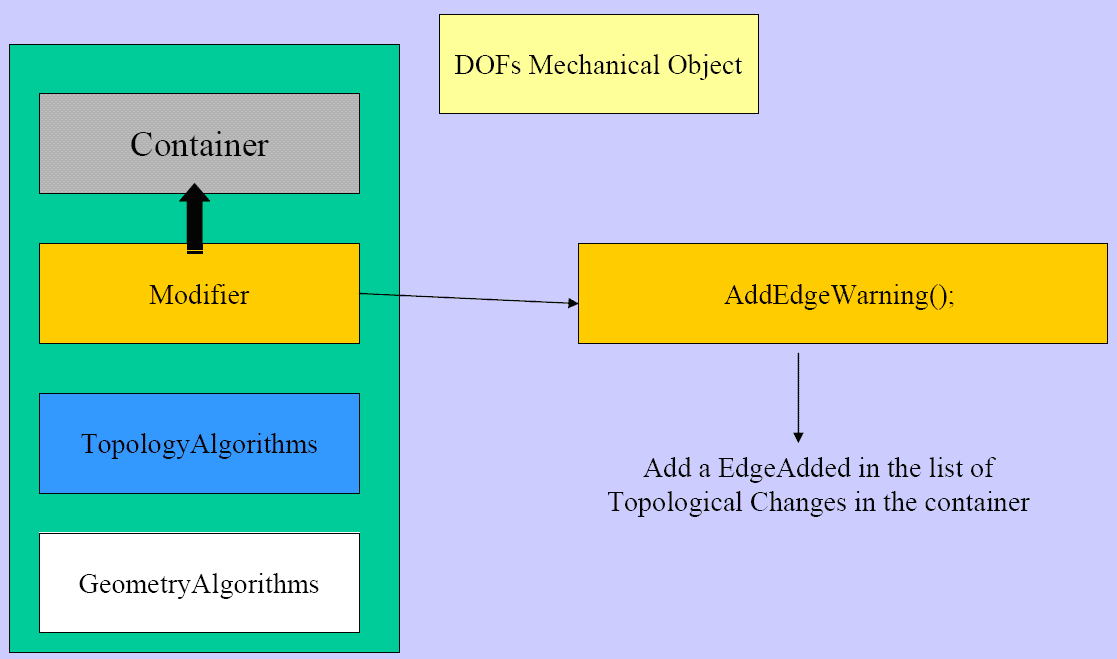
\includegraphics[width=0.9\linewidth]{topology/Topology_Example_6}
  \caption{What happens when I split an Edge ? - Step 5. 6.}
 \label{fig:Topology_Example_56}
\end{figure*}

\newpage

\begin{figure*}[htpb]
 \centering
 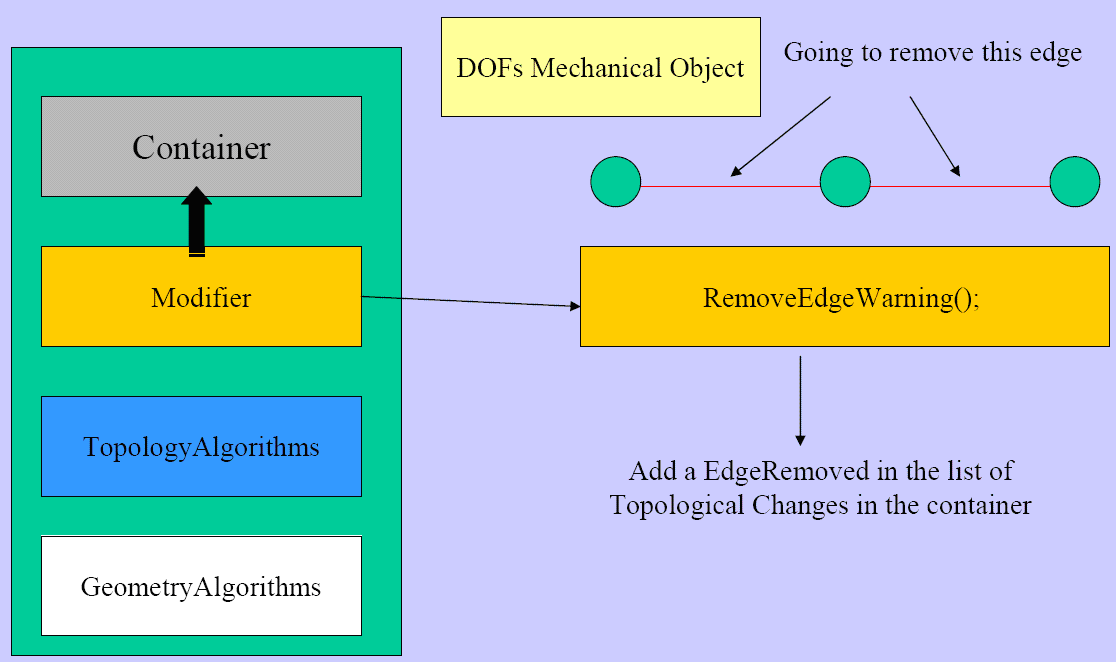
\includegraphics[width=0.9\linewidth]{topology/Topology_Example_7}
 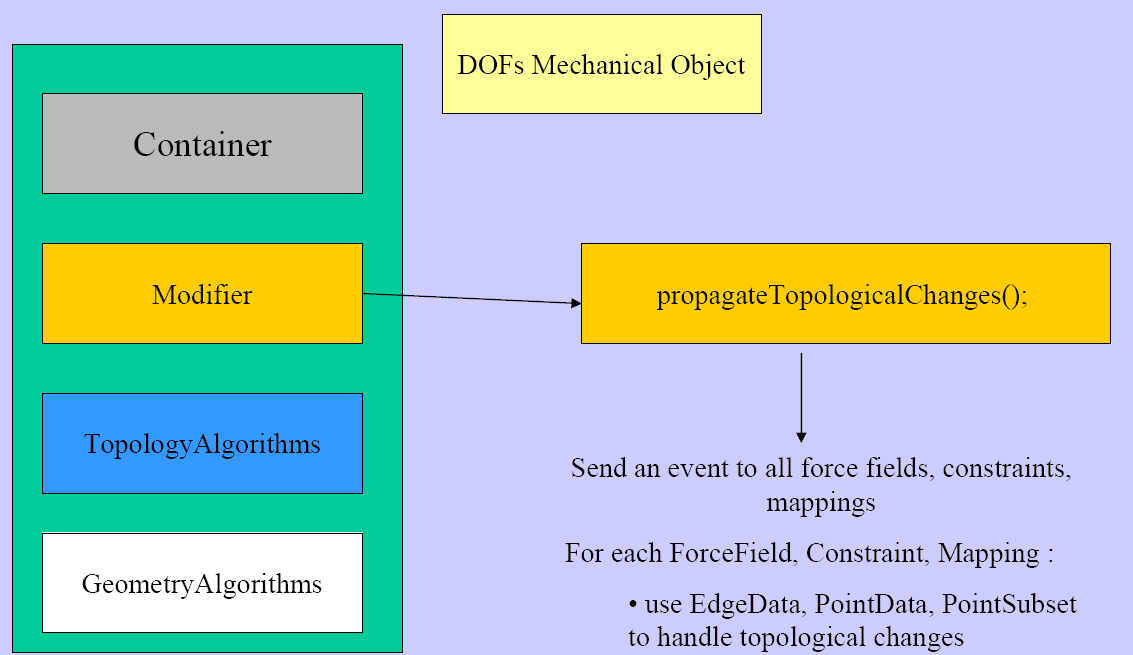
\includegraphics[width=0.9\linewidth]{topology/Topology_Example_8}
  \caption{What happens when I split an Edge ? - Step 7. 8.}
 \label{fig:Topology_Example_78}
\end{figure*}

\newpage

\begin{figure*}[htpb]
 \centering
 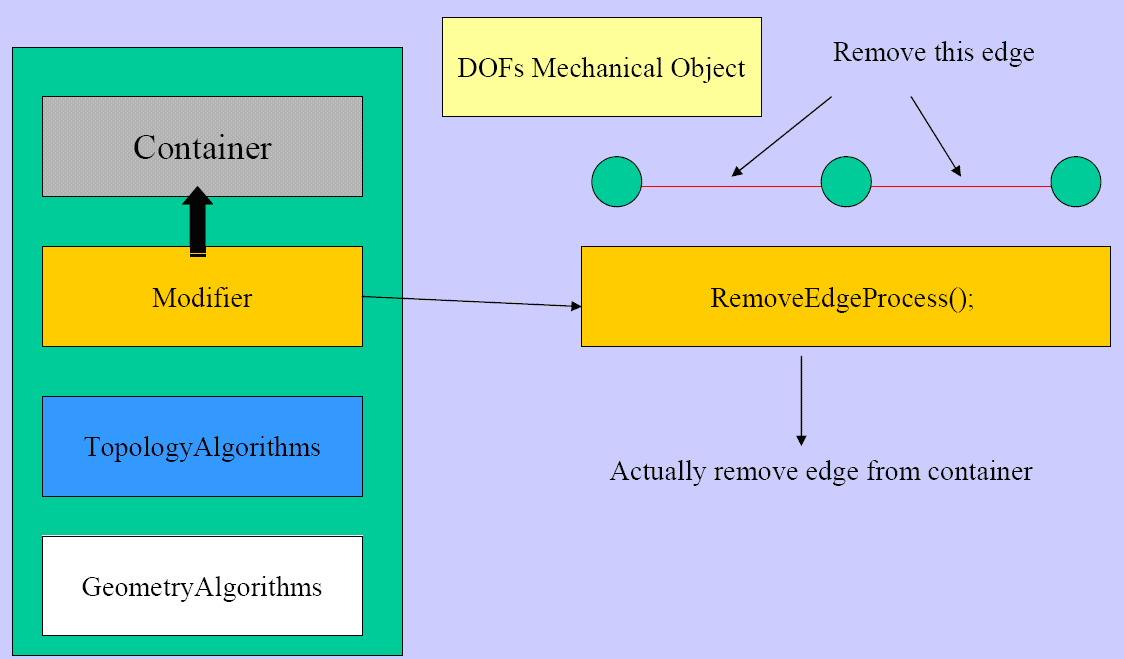
\includegraphics[width=0.9\linewidth]{topology/Topology_Example_9}
  \caption{What happens when I split an Edge ? - Step 9.}
 \label{fig:Topology_Example_9}
\end{figure*}

               
% \subsubsection{Use Cases}


\newpage
\section{Graphic User Interface}
\subsection{First steps}
\par
Once SOFA is compiled, in the directory bin will be placed an executable called runSofa (or runSofad if you are using the debug version).
The first time you will run SOFA, a GUI using Qt will appear. By default a simulation modeling a liver with some fixed points will be displayed. Simulations must be written in a xml format, generally, Sofa scenes have the extension ``.scn'', and Sofa objects directly the extension ``.xml''. You can load both of them using the file menu, or drag \& dropping them in the interface.\\
Basically the GUI is divided in two: 
\begin{itemize}
 \item a control panel subdivided in several tabulations, giving the user the possibility to display various information about the simulation, and even modifying it interactively
 \item a viewer: by default, you will be using our hand-made viewer, using OpenGL. Others are available, and below, we describe how to create your own viewer, if you desire to insert a more powerful rendering engine.
\end{itemize}

\begin{figure}[htpb]
	\centering
		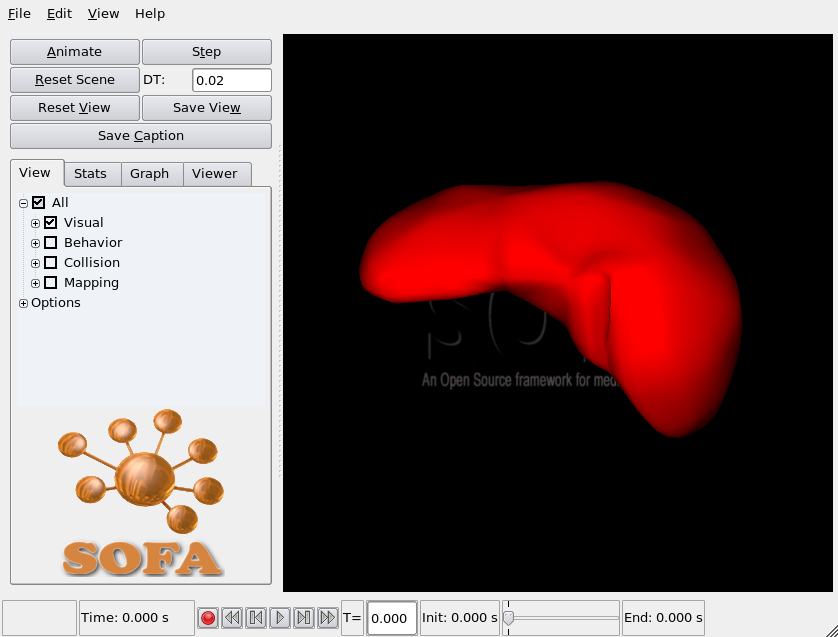
\includegraphics[width=1.0\textwidth]{GUI/GUI.png}
	\caption{SOFA first-time}
\end{figure}
At any time, you can hide the control panel by moving its right border to the left.
\newline

\par

\begin{figure}
	\centering
		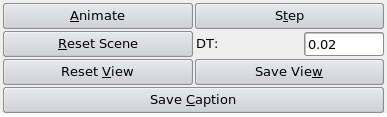
\includegraphics[width=0.45\textwidth]{GUI/GUI_basic.png}
	\caption{Basic Controls}
\end{figure}\begin{center}

\vspace{25mm}            \end{center}
The basics controls are :
\begin{itemize}
 \item {\bf Animate} : launch the simulation. The simulation won't stop until you press Animate.
 \item {\bf Step}: Process only one step of the simulation. 
 \item {\bf Reset Scene}: Reset all the components to their initial values.
 \item {\bf Reset View}: Reset the camera to its original place.
 \item {\bf Save View}: Save the position and orientation of the camera. Next time you will load your scene, these information will be used.
 \item {\bf Save Caption}: Take a screenshot of the current simulation.
\end{itemize}

DT corresponds to the time step used in the computation of the simulation. It can be changed interactively.










\subsection{View Tab}
The ``View Tab'' is the default tab, you can filter the information you want to be displayed by your viewer. It is quite useful to have a fast and global control. 

\begin{figure}[htpb]
	\centering
		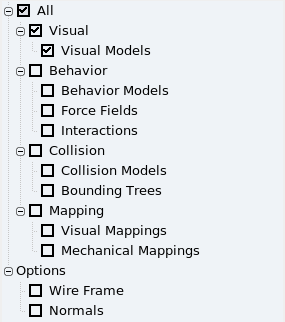
\includegraphics[width=0.3\textwidth]{GUI/GUI_visual.png}
	\caption{Basic Controls}
\end{figure}

The options are:
\begin{itemize}
 \item {\bf All}: Enable or disable the display of all the visual information available in SOFA
 \item {\bf Visual Models}: the graphic representation of the objects
\item {\bf Behavior Models}: the mechanical DOFs of the simulation
\item {\bf Collision Models}: the models used to perform the collision detection
\item {\bf Bounding Tree}: the hierarchical bounding boxes of the collision models
\item {\bf Mappings}: All the non-mechanical mappings (for instance the visual mappings that link a mechanical object to its visual representation)
\item {\bf Mechanical Mappings}: All the mechanical mapping that propagates the forces and position from a mechanical object to another
\item {\bf Interactions}: Interactions of all kind between objects. Some are created by the collision pipeline when a penalty response is used
\item {\bf Wire Frame}: Change the way 3D models(visual, and collision) are displayed
\item {\bf Normals}: Normals of the visual models
\end{itemize}








\subsection{Stats Tab}
The ``Stats Tab'' is a tab displaying an inventory of the collision models present in the scene( how many triangles, lines, points, spheres, are used to perform the collision detection). You can also output some information about the current simulation. 
\begin{itemize}
 \item Dump State: export in ``dumpState.data'' the state of the simulation
 \item Log Time: display in the console, the time spent in each step of the simulation. Useful to do some monitoring
 \item Gnuplot: export gnuplot files. It will export positions, velocities, energies. Files will have the same name as the Object associated in the simulation, following by:
\begin{itemize}
 \item {\bf ``\_x''} for the positions
 \item {\bf ``\_v''} for the velocities
 \item {\bf ``\_Energy''} for the Energies (contains kinetic, potential and mechanical)
\end{itemize}

You can specify the directory where you want the files to be saved in the menu Edit.
\end{itemize}











\subsection{Graph Tab}
The ``Graph tab'' is certainly the most important tab. It displays the scene graph of the simulation. You can quickly see all the components used in the current simulation. The ``Export Graph...'' button gives a graphic representation of the inter-dependencies of the objects.

\begin{figure}[htpb]
	\centering
		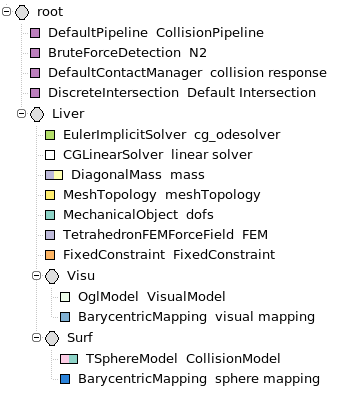
\includegraphics[width=0.5\textwidth]{GUI/GUI_graph.png}
	\caption{Scene Graph for the liver scene}
\end{figure}

This graph can dynamically change during the simulation: collisions can create new nodes, new components in case of contacts. But you can directly interact with it too. Double clicking on an item of the graph will make appear a small window displaying important data.

To know how to display the information of your brand new Sofa component, please refer to the section ``How to configure your Component''. Only objects of type ``sofa::core::objectmodel::Data'' or ``sofa::core::objectmodel::DataPtr'' can be displayed. It is important to understand that only these information will be kept if you decide to save the simulation. Loading a saved simulation, will just fill the components with these datas.
This kind of dialog windows give the possibility to modify directly some characteristics of your component. Take care of clicking on the button ``Update'' once you have completed your modifications.

\begin{figure}[htpb]
	\centering
		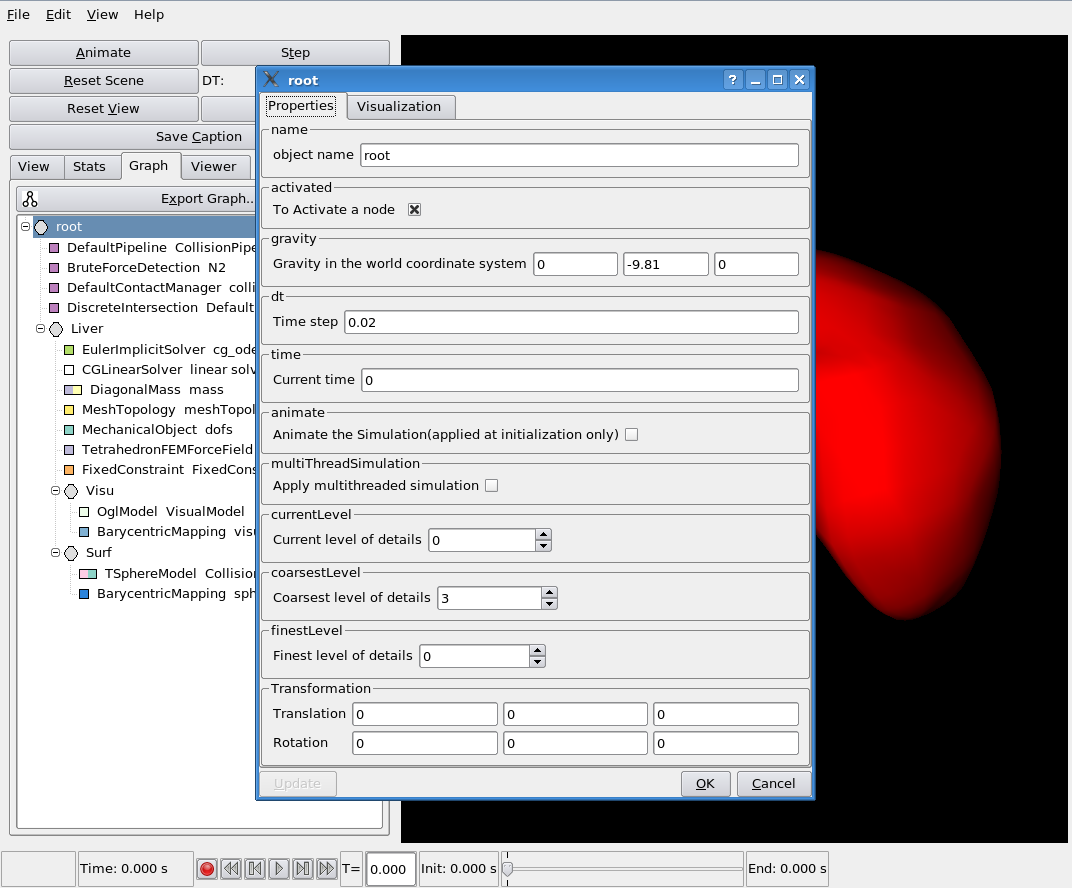
\includegraphics[width=0.8\textwidth]{GUI/GUI_modify.png}
	\caption{Double click on an item of the graph}
\end{figure}

\par
A Node gives access to much more interactions: right clicking on one of them makes appear a small context window.
\begin{itemize}
 \item {\bf Collapse}: Collapse the graph from the current node, so that remain visible the other Nodes and the components right below
 \item {\bf Expand}: Expand the graph, and open all the nodes below the clicked one
 \item {\bf Desactivate}: Desactivate a part of the scene. Everything below this node won't be anymore taken into account. BUT it remains in the scene, and can be Activated again at any time
 \item {\bf Save Node}: Export in a XML files a part of the simulation
 \item {\bf Add Node}: Read a XML files describing an object or a whole scene, and put it right below the clicked node.
An interesting feature to note, is when you might be always using, and adding the same set of objects, you will find it convenient to add in the file scenes/object.txt the path to them. Like this, they will directly appear in the dialog window by default.
 \item {\bf Remove Node}: Remove from the simulation everything within the clicked node. You won't be able anymore to make it appear unless you proceed to a restart or reload of the scene.
 \item {\bf Modify}: Open the same dialog window as might do a double click: this action is common to all the items of the graph
\end{itemize}

\begin{figure}[htpb]
	\centering
		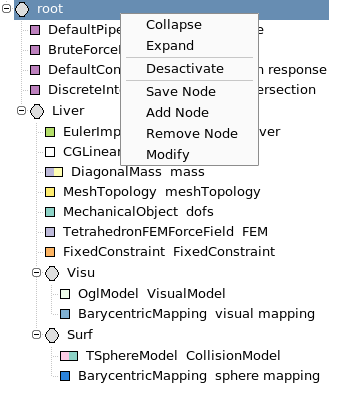
\includegraphics[width=0.4\textwidth]{GUI/GUI_interaction.png}
	\caption{Right click on a node of the graph}
\end{figure}








\subsection{Viewer Tab}
The ``Viewer tab'' describes all the keyboard shortcuts available for the current viewer.

The last useful option of this tab is the possibility to re-size your viewer, which can be very helpful to record a video at a given resolution.









\subsection{Interactions}
You can interact with the simulation using the mouse with SHIFT + Right Click. A ray will be cast, and if it intersects one collision model of the scene, a spring will be created, allowing you to pull on some elements of the scene.



\newpage
\subsection{Architecture}
Fig.~\ref{fig:GUI_UML} gives an overview of the modular architecture of the GUI for SOFA. 
\begin{figure}[htpb]
	\centering
		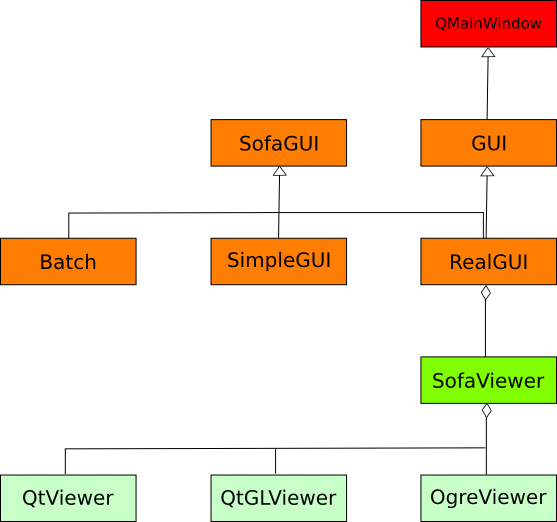
\includegraphics[width=0.9\textwidth]{GUI/GUI_UML.png}
	\caption{A modular Architecture of the GUI}
 	\label{fig:GUI_UML}
\end{figure}








\subsection{Change the viewer}
By default, SOFA provides three viewers, that can be integrated easily to the Qt interface. 

\begin{itemize}
 \item {\bf QtViewer}: a hand made viewer using OpenGL functionality
 \item {\bf QtGLViewer}: a viewer using the library QGLViewer created by Gilles Debunne. It is distributed directly with SOFA, but you can also download it at:\\ {\bf http://artis.imag.fr/Members/Gilles.Debunne/QGLViewer/}
 \item {\bf OgreViewer}: this viewer remains experimental, but shows how it is possible to integrate a powerful rendering engine such as OGRE3D. You need to install Ogre. You can download it at {\bf http://www.ogre3d.org}.
\end{itemize}

To use them, you have to edit the file sofa-default.cfg located in your SOFA directory, and uncomment the lines corresponding to the viewer you want. If you have several viewers activated, you can launch SOFA with a specific one by using the option:
\begin{itemize}
 \item ``runSofa -g qt'' : for QtViewer
 \item ``runSofa -g qglviewer'' : for QtGLViewer
 \item ``runSofa -g ogre'' : for OgreViewer
\end{itemize}

You can also dynamically change the viewer when SOFA is running. The menu View of the main window displays all the viewer available and let you switch at any time.
\par
If you desire to create a new viewer, the first step is to make it derive from SofaViewer. 








\subsection{Choose the GUI}
By default, Sofa provides three GUIs.
\begin{itemize}
 \item {\bf Batch}: no gui, proceeds to 1000 iterations and then stops
 \item {\bf GLUT}: GLUT window, implementing only the basic functions. To start the animation, you have to pass the option ``-s'' to your runSofa
 \item {\bf Qt}: the default GUI, already described above
\end{itemize}

The Batch GUI is always available. To use GLUT or Qt interface, you have to uncomment in sofa-default.cfg the corresponding lines. To use them
\begin{itemize}
 \item ``runSofa -g batch'' : for no GUI
 \item ``runSofa -g glut'' : for GLUT window 
 \item for Qt GUI, please refer to the section above. By default, Sofa is using Qt interface with QtViewer.
\end{itemize}
If you desire to create a new GUI, the first step is to make it derive from SofaGUI. 






\subsection{Player/Recorder}

\begin{figure}[htpb]
	\centering
		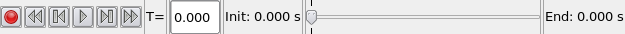
\includegraphics[width=0.7\textwidth]{GUI/GUI_recorder.png}
	\caption{Player/Recorder in Sofa} 	
\end{figure}
Sofa provides with the Qt Graphic interface, a compact Player/Recorder of simulation. When you want to record a simulation, press the red button (record). Automatically, some components will be added to your graph, and will create files to save the position, and velocities of all your mechanical elements. To stop recording, press again on the record button. A file with the same name as your simulation will be created, but with the extension ``.simu''. Sofa is able to read these files, and will initialize correctly the Player. 
\par
To readback a recorded simulation, you can process to a step by step(forward, and backward), or a continuous play. You can jump to a specific moment of your recording. You can even change the Dt of the recording, if you want to accelerate, or reduce the velocity of the playing. At any time, you can animate the scene (by pressing the Animate button), to compute the simulation. 
\par
The files will be stored by default in the directory scenes/simulation of your SOFA. Nevertheless, you can change this directory by clicking on the menu Edit of the main window.







\section{Modeler}
A modeler for Sofa has been recently created. The purpose of this tool is both to help the new-comers in Sofa to get an overview of the whole framework, and accelerate the process of creation and configuration of a complex simulation for expert users.
\begin{figure}[htpb]
	\centering
		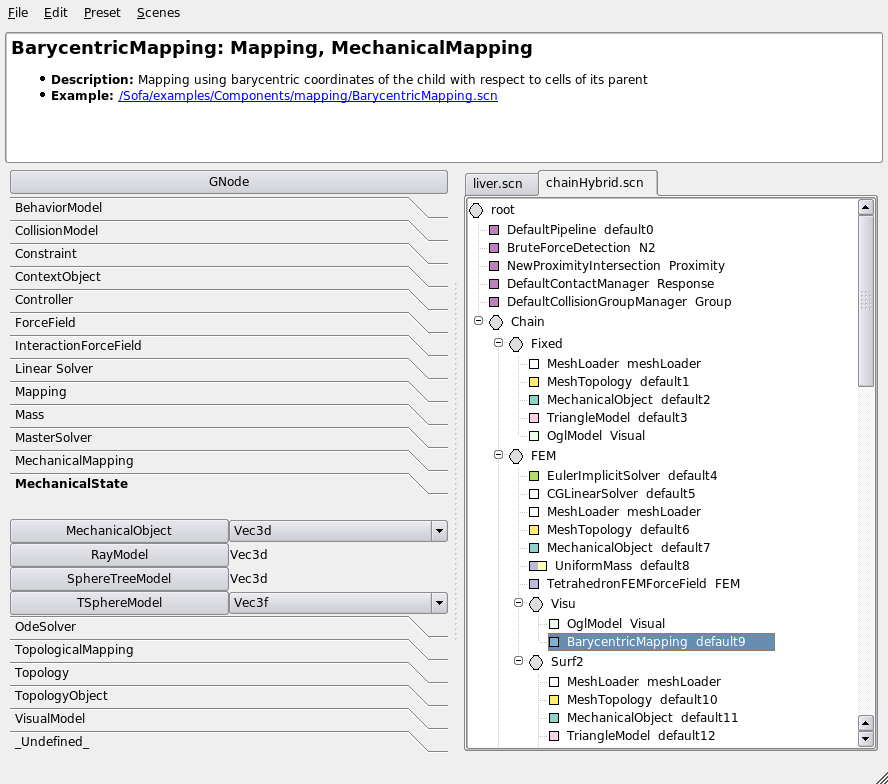
\includegraphics[width=0.75\textwidth]{GUI/Modeler.png}
	\caption{Main Window of the Modeler} 	
\end{figure}

\subsection{Library}
The left part of the application displays a library of all the different components available in Sofa, sorted by the name of the Base Class. Clicking on any of them will display information about the usage, authors, licence if any, and sometimes a link to an example. This link will open a new tab in the modeler displaying a simulation. 
At any time, you can launch Sofa from the Modeler, hitting CTRL+R, or going to File ... Run In Sofa.
\subsection{Graph Editor}
The right part seems very similar to the scene graph displayed in Sofa. The behavior is the same. Double clicking on a component will open a dialog, in which you can define all the parameters of the object. But, as you are in an editor, you can easily remove everything you have added. This editor is very convenient to test things. Try to create your object, launch into sofa, modify some components, or parameters, using the documentation displayed each time you select one item. 
\subsection{Modeling}
To model a new scene, just make a series of drag and drop of the components you desire from the Library to the Graph Editor. By default, when opening a new tab, all the default components to perform the collision detection are added. If you don't want them, just clear the tab (CTRL+N).\\
To accelerate the process of creation, preset objects are available. You can build automatically :
\begin{itemize}
  \item deformable objects
  \begin{itemize}
    \item in a grid
    \item using a tetrahedral mesh
  \end{itemize}
  \item rigid objects  
  \begin{itemize}
    \item simulated
    \item not simulated: they will perform as obstacle like floors, or walls
  \end{itemize}
\end{itemize}




\end{document}          

